% Created by tikzDevice version 0.7.0 on 2014-11-11 22:06:21
% !TEX encoding = UTF-8 Unicode
\documentclass[tikz]{standalone}

\begin{document}

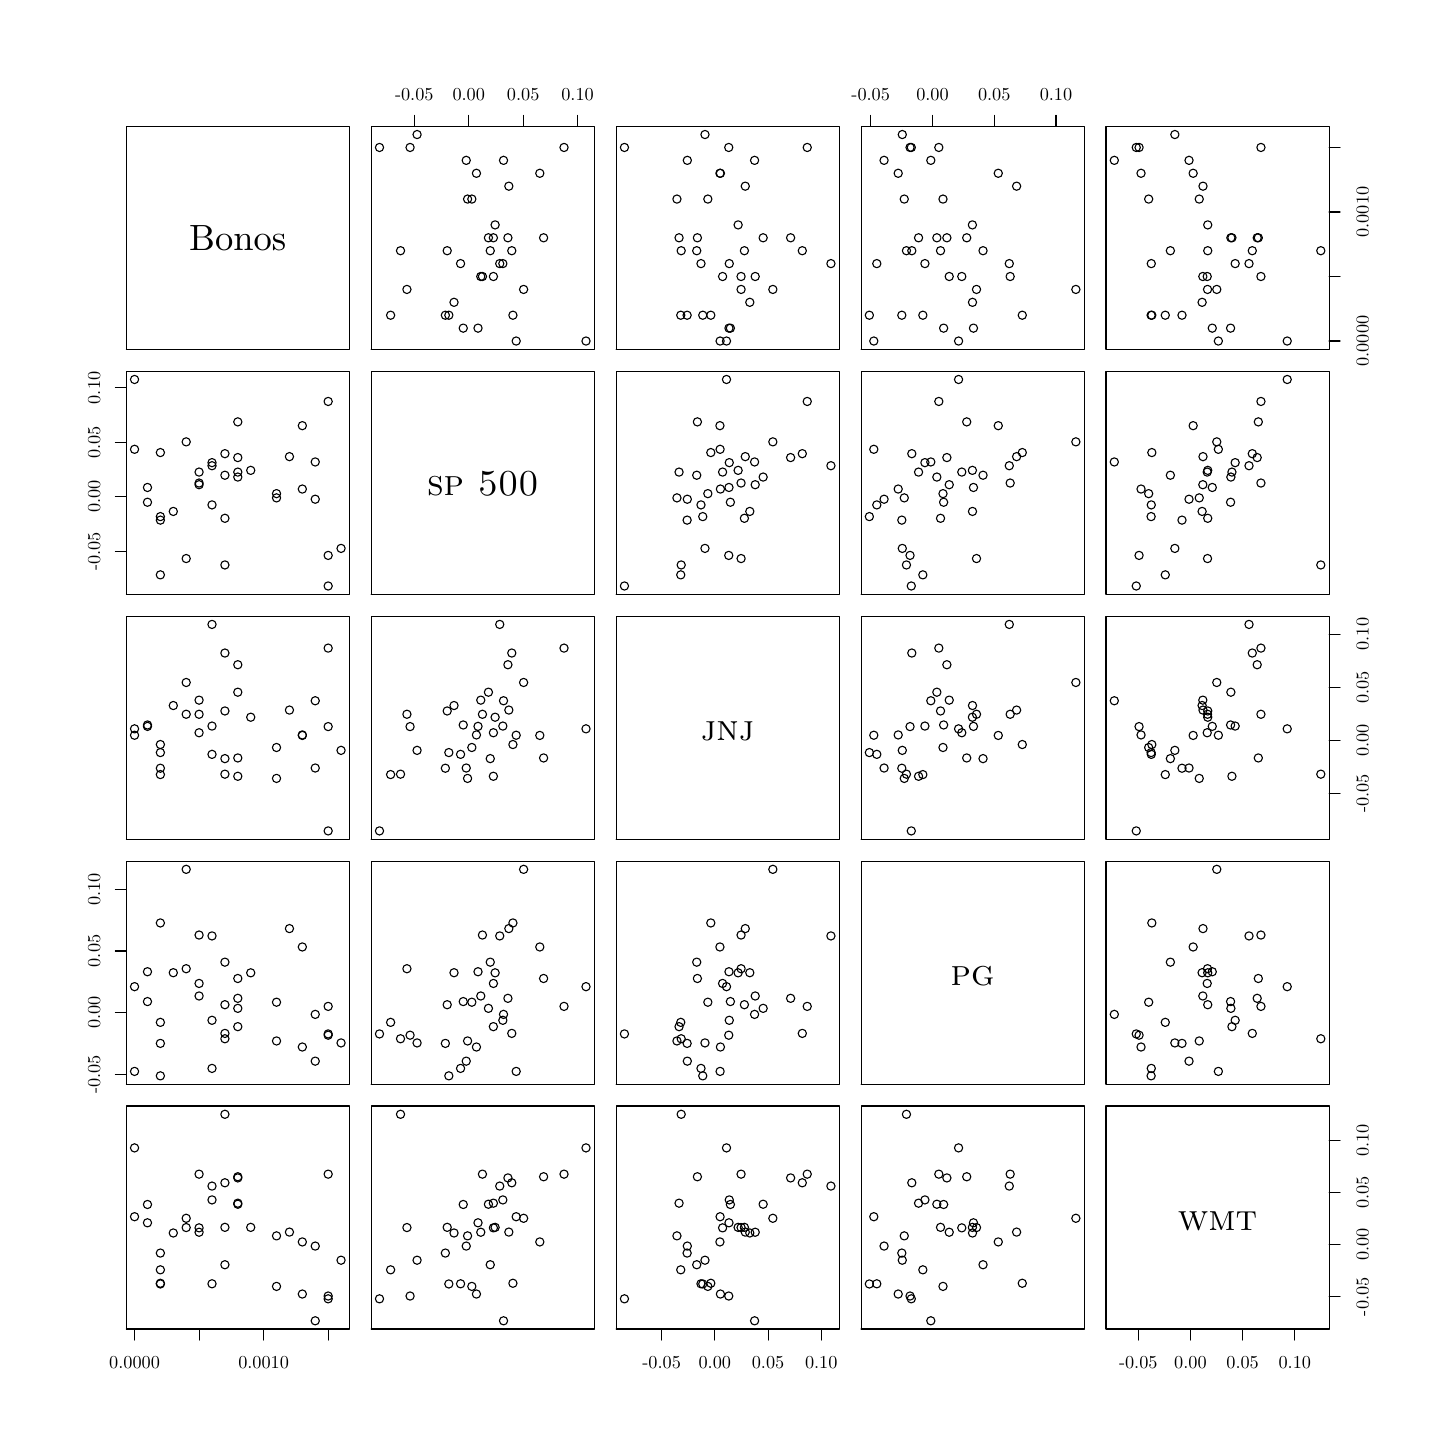
\begin{tikzpicture}[x=1pt,y=1pt]
\definecolor[named]{fillColor}{rgb}{1.00,1.00,1.00}
\path[use as bounding box,fill=fillColor,fill opacity=0.00] (0,0) rectangle (505.89,505.89);
\begin{scope}
\path[clip] (  0.00,  0.00) rectangle (505.89,505.89);
\definecolor[named]{drawColor}{rgb}{0.00,0.00,0.00}

\path[draw=drawColor,line width= 0.4pt,line join=round,line cap=round] ( 35.64,389.66) --
	(116.23,389.66) --
	(116.23,470.25) --
	( 35.64,470.25) --
	( 35.64,389.66);
\end{scope}
\begin{scope}
\path[clip] ( 35.64,389.66) rectangle (116.23,470.25);
\definecolor[named]{drawColor}{rgb}{0.00,0.00,0.00}

\node[text=drawColor,anchor=base,inner sep=0pt, outer sep=0pt, scale=  1.32] at ( 75.93,425.41) {Bonos};
\end{scope}
\begin{scope}
\path[clip] (  0.00,  0.00) rectangle (505.89,505.89);
\definecolor[named]{drawColor}{rgb}{0.00,0.00,0.00}

\path[draw=drawColor,line width= 0.4pt,line join=round,line cap=round] (124.15,389.66) --
	(204.73,389.66) --
	(204.73,470.25) --
	(124.15,470.25) --
	(124.15,389.66);

\path[draw=drawColor,line width= 0.4pt,line join=round,line cap=round] (139.71,470.25) -- (198.71,470.25);

\path[draw=drawColor,line width= 0.4pt,line join=round,line cap=round] (139.71,470.25) -- (139.71,474.21);

\path[draw=drawColor,line width= 0.4pt,line join=round,line cap=round] (159.38,470.25) -- (159.38,474.21);

\path[draw=drawColor,line width= 0.4pt,line join=round,line cap=round] (179.04,470.25) -- (179.04,474.21);

\path[draw=drawColor,line width= 0.4pt,line join=round,line cap=round] (198.71,470.25) -- (198.71,474.21);

\node[text=drawColor,anchor=base,inner sep=0pt, outer sep=0pt, scale=  0.66] at (139.71,479.75) {-0.05};

\node[text=drawColor,anchor=base,inner sep=0pt, outer sep=0pt, scale=  0.66] at (159.38,479.75) {0.00};

\node[text=drawColor,anchor=base,inner sep=0pt, outer sep=0pt, scale=  0.66] at (179.04,479.75) {0.05};

\node[text=drawColor,anchor=base,inner sep=0pt, outer sep=0pt, scale=  0.66] at (198.71,479.75) {0.10};
\end{scope}
\begin{scope}
\path[clip] (124.15,389.66) rectangle (204.73,470.25);
\definecolor[named]{drawColor}{rgb}{0.00,0.00,0.00}

\path[draw=drawColor,line width= 0.4pt,line join=round,line cap=round] (127.13,462.60) circle (  1.49);

\path[draw=drawColor,line width= 0.4pt,line join=round,line cap=round] (138.18,462.60) circle (  1.49);

\path[draw=drawColor,line width= 0.4pt,line join=round,line cap=round] (186.43,429.96) circle (  1.49);

\path[draw=drawColor,line width= 0.4pt,line join=round,line cap=round] (140.71,467.27) circle (  1.49);

\path[draw=drawColor,line width= 0.4pt,line join=round,line cap=round] (193.81,462.60) circle (  1.49);

\path[draw=drawColor,line width= 0.4pt,line join=round,line cap=round] (173.87,448.61) circle (  1.49);

\path[draw=drawColor,line width= 0.4pt,line join=round,line cap=round] (158.47,457.94) circle (  1.49);

\path[draw=drawColor,line width= 0.4pt,line join=round,line cap=round] (185.06,453.27) circle (  1.49);

\path[draw=drawColor,line width= 0.4pt,line join=round,line cap=round] (168.28,429.96) circle (  1.49);

\path[draw=drawColor,line width= 0.4pt,line join=round,line cap=round] (171.95,457.94) circle (  1.49);

\path[draw=drawColor,line width= 0.4pt,line join=round,line cap=round] (158.96,443.95) circle (  1.49);

\path[draw=drawColor,line width= 0.4pt,line join=round,line cap=round] (170.58,420.63) circle (  1.49);

\path[draw=drawColor,line width= 0.4pt,line join=round,line cap=round] (154.06,406.64) circle (  1.49);

\path[draw=drawColor,line width= 0.4pt,line join=round,line cap=round] (152.19,401.98) circle (  1.49);

\path[draw=drawColor,line width= 0.4pt,line join=round,line cap=round] (150.93,401.98) circle (  1.49);

\path[draw=drawColor,line width= 0.4pt,line join=round,line cap=round] (137.04,411.30) circle (  1.49);

\path[draw=drawColor,line width= 0.4pt,line join=round,line cap=round] (131.15,401.98) circle (  1.49);

\path[draw=drawColor,line width= 0.4pt,line join=round,line cap=round] (201.75,392.65) circle (  1.49);

\path[draw=drawColor,line width= 0.4pt,line join=round,line cap=round] (157.39,397.31) circle (  1.49);

\path[draw=drawColor,line width= 0.4pt,line join=round,line cap=round] (162.73,397.31) circle (  1.49);

\path[draw=drawColor,line width= 0.4pt,line join=round,line cap=round] (176.52,392.65) circle (  1.49);

\path[draw=drawColor,line width= 0.4pt,line join=round,line cap=round] (175.34,401.98) circle (  1.49);

\path[draw=drawColor,line width= 0.4pt,line join=round,line cap=round] (171.70,420.63) circle (  1.49);

\path[draw=drawColor,line width= 0.4pt,line join=round,line cap=round] (156.43,420.63) circle (  1.49);

\path[draw=drawColor,line width= 0.4pt,line join=round,line cap=round] (134.73,425.29) circle (  1.49);

\path[draw=drawColor,line width= 0.4pt,line join=round,line cap=round] (174.93,425.29) circle (  1.49);

\path[draw=drawColor,line width= 0.4pt,line join=round,line cap=round] (164.33,415.97) circle (  1.49);

\path[draw=drawColor,line width= 0.4pt,line join=round,line cap=round] (167.15,425.29) circle (  1.49);

\path[draw=drawColor,line width= 0.4pt,line join=round,line cap=round] (168.91,434.62) circle (  1.49);

\path[draw=drawColor,line width= 0.4pt,line join=round,line cap=round] (151.59,425.29) circle (  1.49);

\path[draw=drawColor,line width= 0.4pt,line join=round,line cap=round] (160.50,443.95) circle (  1.49);

\path[draw=drawColor,line width= 0.4pt,line join=round,line cap=round] (162.16,453.27) circle (  1.49);

\path[draw=drawColor,line width= 0.4pt,line join=round,line cap=round] (179.21,411.30) circle (  1.49);

\path[draw=drawColor,line width= 0.4pt,line join=round,line cap=round] (163.73,415.97) circle (  1.49);

\path[draw=drawColor,line width= 0.4pt,line join=round,line cap=round] (173.53,429.96) circle (  1.49);

\path[draw=drawColor,line width= 0.4pt,line join=round,line cap=round] (166.49,429.96) circle (  1.49);

\path[draw=drawColor,line width= 0.4pt,line join=round,line cap=round] (168.29,415.97) circle (  1.49);
\end{scope}
\begin{scope}
\path[clip] (  0.00,  0.00) rectangle (505.89,505.89);
\definecolor[named]{drawColor}{rgb}{0.00,0.00,0.00}

\path[draw=drawColor,line width= 0.4pt,line join=round,line cap=round] (212.65,389.66) --
	(293.24,389.66) --
	(293.24,470.25) --
	(212.65,470.25) --
	(212.65,389.66);
\end{scope}
\begin{scope}
\path[clip] (212.65,389.66) rectangle (293.24,470.25);
\definecolor[named]{drawColor}{rgb}{0.00,0.00,0.00}

\path[draw=drawColor,line width= 0.4pt,line join=round,line cap=round] (215.64,462.60) circle (  1.49);

\path[draw=drawColor,line width= 0.4pt,line join=round,line cap=round] (253.33,462.60) circle (  1.49);

\path[draw=drawColor,line width= 0.4pt,line join=round,line cap=round] (242.00,429.96) circle (  1.49);

\path[draw=drawColor,line width= 0.4pt,line join=round,line cap=round] (244.74,467.27) circle (  1.49);

\path[draw=drawColor,line width= 0.4pt,line join=round,line cap=round] (281.69,462.60) circle (  1.49);

\path[draw=drawColor,line width= 0.4pt,line join=round,line cap=round] (259.30,448.61) circle (  1.49);

\path[draw=drawColor,line width= 0.4pt,line join=round,line cap=round] (238.36,457.94) circle (  1.49);

\path[draw=drawColor,line width= 0.4pt,line join=round,line cap=round] (250.14,453.27) circle (  1.49);

\path[draw=drawColor,line width= 0.4pt,line join=round,line cap=round] (235.38,429.96) circle (  1.49);

\path[draw=drawColor,line width= 0.4pt,line join=round,line cap=round] (262.67,457.94) circle (  1.49);

\path[draw=drawColor,line width= 0.4pt,line join=round,line cap=round] (234.61,443.95) circle (  1.49);

\path[draw=drawColor,line width= 0.4pt,line join=round,line cap=round] (290.25,420.63) circle (  1.49);

\path[draw=drawColor,line width= 0.4pt,line join=round,line cap=round] (260.94,406.64) circle (  1.49);

\path[draw=drawColor,line width= 0.4pt,line join=round,line cap=round] (243.94,401.98) circle (  1.49);

\path[draw=drawColor,line width= 0.4pt,line join=round,line cap=round] (238.29,401.98) circle (  1.49);

\path[draw=drawColor,line width= 0.4pt,line join=round,line cap=round] (257.79,411.30) circle (  1.49);

\path[draw=drawColor,line width= 0.4pt,line join=round,line cap=round] (235.99,401.98) circle (  1.49);

\path[draw=drawColor,line width= 0.4pt,line join=round,line cap=round] (252.52,392.65) circle (  1.49);

\path[draw=drawColor,line width= 0.4pt,line join=round,line cap=round] (253.92,397.31) circle (  1.49);

\path[draw=drawColor,line width= 0.4pt,line join=round,line cap=round] (253.41,397.31) circle (  1.49);

\path[draw=drawColor,line width= 0.4pt,line join=round,line cap=round] (250.21,392.65) circle (  1.49);

\path[draw=drawColor,line width= 0.4pt,line join=round,line cap=round] (246.85,401.98) circle (  1.49);

\path[draw=drawColor,line width= 0.4pt,line join=round,line cap=round] (253.52,420.63) circle (  1.49);

\path[draw=drawColor,line width= 0.4pt,line join=round,line cap=round] (243.30,420.63) circle (  1.49);

\path[draw=drawColor,line width= 0.4pt,line join=round,line cap=round] (236.14,425.29) circle (  1.49);

\path[draw=drawColor,line width= 0.4pt,line join=round,line cap=round] (279.91,425.29) circle (  1.49);

\path[draw=drawColor,line width= 0.4pt,line join=round,line cap=round] (257.78,415.97) circle (  1.49);

\path[draw=drawColor,line width= 0.4pt,line join=round,line cap=round] (241.76,425.29) circle (  1.49);

\path[draw=drawColor,line width= 0.4pt,line join=round,line cap=round] (256.72,434.62) circle (  1.49);

\path[draw=drawColor,line width= 0.4pt,line join=round,line cap=round] (258.98,425.29) circle (  1.49);

\path[draw=drawColor,line width= 0.4pt,line join=round,line cap=round] (245.78,443.95) circle (  1.49);

\path[draw=drawColor,line width= 0.4pt,line join=round,line cap=round] (250.32,453.27) circle (  1.49);

\path[draw=drawColor,line width= 0.4pt,line join=round,line cap=round] (269.27,411.30) circle (  1.49);

\path[draw=drawColor,line width= 0.4pt,line join=round,line cap=round] (262.89,415.97) circle (  1.49);

\path[draw=drawColor,line width= 0.4pt,line join=round,line cap=round] (275.69,429.96) circle (  1.49);

\path[draw=drawColor,line width= 0.4pt,line join=round,line cap=round] (265.76,429.96) circle (  1.49);

\path[draw=drawColor,line width= 0.4pt,line join=round,line cap=round] (251.11,415.97) circle (  1.49);
\end{scope}
\begin{scope}
\path[clip] (  0.00,  0.00) rectangle (505.89,505.89);
\definecolor[named]{drawColor}{rgb}{0.00,0.00,0.00}

\path[draw=drawColor,line width= 0.4pt,line join=round,line cap=round] (301.16,389.66) --
	(381.74,389.66) --
	(381.74,470.25) --
	(301.16,470.25) --
	(301.16,389.66);

\path[draw=drawColor,line width= 0.4pt,line join=round,line cap=round] (304.64,470.25) -- (371.58,470.25);

\path[draw=drawColor,line width= 0.4pt,line join=round,line cap=round] (304.64,470.25) -- (304.64,474.21);

\path[draw=drawColor,line width= 0.4pt,line join=round,line cap=round] (326.96,470.25) -- (326.96,474.21);

\path[draw=drawColor,line width= 0.4pt,line join=round,line cap=round] (349.27,470.25) -- (349.27,474.21);

\path[draw=drawColor,line width= 0.4pt,line join=round,line cap=round] (371.58,470.25) -- (371.58,474.21);

\node[text=drawColor,anchor=base,inner sep=0pt, outer sep=0pt, scale=  0.66] at (304.64,479.75) {-0.05};

\node[text=drawColor,anchor=base,inner sep=0pt, outer sep=0pt, scale=  0.66] at (326.96,479.75) {0.00};

\node[text=drawColor,anchor=base,inner sep=0pt, outer sep=0pt, scale=  0.66] at (349.27,479.75) {0.05};

\node[text=drawColor,anchor=base,inner sep=0pt, outer sep=0pt, scale=  0.66] at (371.58,479.75) {0.10};
\end{scope}
\begin{scope}
\path[clip] (301.16,389.66) rectangle (381.74,470.25);
\definecolor[named]{drawColor}{rgb}{0.00,0.00,0.00}

\path[draw=drawColor,line width= 0.4pt,line join=round,line cap=round] (319.29,462.60) circle (  1.49);

\path[draw=drawColor,line width= 0.4pt,line join=round,line cap=round] (318.84,462.60) circle (  1.49);

\path[draw=drawColor,line width= 0.4pt,line join=round,line cap=round] (339.32,429.96) circle (  1.49);

\path[draw=drawColor,line width= 0.4pt,line join=round,line cap=round] (316.04,467.27) circle (  1.49);

\path[draw=drawColor,line width= 0.4pt,line join=round,line cap=round] (329.24,462.60) circle (  1.49);

\path[draw=drawColor,line width= 0.4pt,line join=round,line cap=round] (357.35,448.61) circle (  1.49);

\path[draw=drawColor,line width= 0.4pt,line join=round,line cap=round] (309.46,457.94) circle (  1.49);

\path[draw=drawColor,line width= 0.4pt,line join=round,line cap=round] (350.72,453.27) circle (  1.49);

\path[draw=drawColor,line width= 0.4pt,line join=round,line cap=round] (321.92,429.96) circle (  1.49);

\path[draw=drawColor,line width= 0.4pt,line join=round,line cap=round] (326.35,457.94) circle (  1.49);

\path[draw=drawColor,line width= 0.4pt,line join=round,line cap=round] (316.75,443.95) circle (  1.49);

\path[draw=drawColor,line width= 0.4pt,line join=round,line cap=round] (354.70,420.63) circle (  1.49);

\path[draw=drawColor,line width= 0.4pt,line join=round,line cap=round] (341.41,406.64) circle (  1.49);

\path[draw=drawColor,line width= 0.4pt,line join=round,line cap=round] (304.14,401.98) circle (  1.49);

\path[draw=drawColor,line width= 0.4pt,line join=round,line cap=round] (315.87,401.98) circle (  1.49);

\path[draw=drawColor,line width= 0.4pt,line join=round,line cap=round] (342.86,411.30) circle (  1.49);

\path[draw=drawColor,line width= 0.4pt,line join=round,line cap=round] (323.47,401.98) circle (  1.49);

\path[draw=drawColor,line width= 0.4pt,line join=round,line cap=round] (336.38,392.65) circle (  1.49);

\path[draw=drawColor,line width= 0.4pt,line join=round,line cap=round] (330.98,397.31) circle (  1.49);

\path[draw=drawColor,line width= 0.4pt,line join=round,line cap=round] (341.76,397.31) circle (  1.49);

\path[draw=drawColor,line width= 0.4pt,line join=round,line cap=round] (305.75,392.65) circle (  1.49);

\path[draw=drawColor,line width= 0.4pt,line join=round,line cap=round] (359.40,401.98) circle (  1.49);

\path[draw=drawColor,line width= 0.4pt,line join=round,line cap=round] (324.21,420.63) circle (  1.49);

\path[draw=drawColor,line width= 0.4pt,line join=round,line cap=round] (306.83,420.63) circle (  1.49);

\path[draw=drawColor,line width= 0.4pt,line join=round,line cap=round] (317.54,425.29) circle (  1.49);

\path[draw=drawColor,line width= 0.4pt,line join=round,line cap=round] (319.48,425.29) circle (  1.49);

\path[draw=drawColor,line width= 0.4pt,line join=round,line cap=round] (355.02,415.97) circle (  1.49);

\path[draw=drawColor,line width= 0.4pt,line join=round,line cap=round] (345.22,425.29) circle (  1.49);

\path[draw=drawColor,line width= 0.4pt,line join=round,line cap=round] (341.37,434.62) circle (  1.49);

\path[draw=drawColor,line width= 0.4pt,line join=round,line cap=round] (329.86,425.29) circle (  1.49);

\path[draw=drawColor,line width= 0.4pt,line join=round,line cap=round] (330.75,443.95) circle (  1.49);

\path[draw=drawColor,line width= 0.4pt,line join=round,line cap=round] (314.56,453.27) circle (  1.49);

\path[draw=drawColor,line width= 0.4pt,line join=round,line cap=round] (378.76,411.30) circle (  1.49);

\path[draw=drawColor,line width= 0.4pt,line join=round,line cap=round] (333.00,415.97) circle (  1.49);

\path[draw=drawColor,line width= 0.4pt,line join=round,line cap=round] (332.15,429.96) circle (  1.49);

\path[draw=drawColor,line width= 0.4pt,line join=round,line cap=round] (328.53,429.96) circle (  1.49);

\path[draw=drawColor,line width= 0.4pt,line join=round,line cap=round] (337.54,415.97) circle (  1.49);
\end{scope}
\begin{scope}
\path[clip] (  0.00,  0.00) rectangle (505.89,505.89);
\definecolor[named]{drawColor}{rgb}{0.00,0.00,0.00}

\path[draw=drawColor,line width= 0.4pt,line join=round,line cap=round] (389.66,389.66) --
	(470.25,389.66) --
	(470.25,470.25) --
	(389.66,470.25) --
	(389.66,389.66);

\path[draw=drawColor,line width= 0.4pt,line join=round,line cap=round] (470.25,392.65) -- (470.25,462.60);

\path[draw=drawColor,line width= 0.4pt,line join=round,line cap=round] (470.25,392.65) -- (474.21,392.65);

\path[draw=drawColor,line width= 0.4pt,line join=round,line cap=round] (470.25,415.97) -- (474.21,415.97);

\path[draw=drawColor,line width= 0.4pt,line join=round,line cap=round] (470.25,439.28) -- (474.21,439.28);

\path[draw=drawColor,line width= 0.4pt,line join=round,line cap=round] (470.25,462.60) -- (474.21,462.60);

\node[text=drawColor,rotate= 90.00,anchor=base,inner sep=0pt, outer sep=0pt, scale=  0.66] at (484.51,392.65) {0.0000};

\node[text=drawColor,rotate= 90.00,anchor=base,inner sep=0pt, outer sep=0pt, scale=  0.66] at (484.51,439.28) {0.0010};
\end{scope}
\begin{scope}
\path[clip] (389.66,389.66) rectangle (470.25,470.25);
\definecolor[named]{drawColor}{rgb}{0.00,0.00,0.00}

\path[draw=drawColor,line width= 0.4pt,line join=round,line cap=round] (400.58,462.60) circle (  1.49);

\path[draw=drawColor,line width= 0.4pt,line join=round,line cap=round] (401.60,462.60) circle (  1.49);

\path[draw=drawColor,line width= 0.4pt,line join=round,line cap=round] (444.69,429.96) circle (  1.49);

\path[draw=drawColor,line width= 0.4pt,line join=round,line cap=round] (414.53,467.27) circle (  1.49);

\path[draw=drawColor,line width= 0.4pt,line join=round,line cap=round] (445.64,462.60) circle (  1.49);

\path[draw=drawColor,line width= 0.4pt,line join=round,line cap=round] (424.70,448.61) circle (  1.49);

\path[draw=drawColor,line width= 0.4pt,line join=round,line cap=round] (419.65,457.94) circle (  1.49);

\path[draw=drawColor,line width= 0.4pt,line join=round,line cap=round] (421.14,453.27) circle (  1.49);

\path[draw=drawColor,line width= 0.4pt,line join=round,line cap=round] (435.15,429.96) circle (  1.49);

\path[draw=drawColor,line width= 0.4pt,line join=round,line cap=round] (392.65,457.94) circle (  1.49);

\path[draw=drawColor,line width= 0.4pt,line join=round,line cap=round] (423.34,443.95) circle (  1.49);

\path[draw=drawColor,line width= 0.4pt,line join=round,line cap=round] (441.33,420.63) circle (  1.49);

\path[draw=drawColor,line width= 0.4pt,line join=round,line cap=round] (424.38,406.64) circle (  1.49);

\path[draw=drawColor,line width= 0.4pt,line join=round,line cap=round] (405.95,401.98) circle (  1.49);

\path[draw=drawColor,line width= 0.4pt,line join=round,line cap=round] (417.11,401.98) circle (  1.49);

\path[draw=drawColor,line width= 0.4pt,line join=round,line cap=round] (426.34,411.30) circle (  1.49);

\path[draw=drawColor,line width= 0.4pt,line join=round,line cap=round] (411.07,401.98) circle (  1.49);

\path[draw=drawColor,line width= 0.4pt,line join=round,line cap=round] (455.13,392.65) circle (  1.49);

\path[draw=drawColor,line width= 0.4pt,line join=round,line cap=round] (434.67,397.31) circle (  1.49);

\path[draw=drawColor,line width= 0.4pt,line join=round,line cap=round] (428.05,397.31) circle (  1.49);

\path[draw=drawColor,line width= 0.4pt,line join=round,line cap=round] (430.25,392.65) circle (  1.49);

\path[draw=drawColor,line width= 0.4pt,line join=round,line cap=round] (406.21,401.98) circle (  1.49);

\path[draw=drawColor,line width= 0.4pt,line join=round,line cap=round] (436.32,420.63) circle (  1.49);

\path[draw=drawColor,line width= 0.4pt,line join=round,line cap=round] (406.01,420.63) circle (  1.49);

\path[draw=drawColor,line width= 0.4pt,line join=round,line cap=round] (467.27,425.29) circle (  1.49);

\path[draw=drawColor,line width= 0.4pt,line join=round,line cap=round] (442.51,425.29) circle (  1.49);

\path[draw=drawColor,line width= 0.4pt,line join=round,line cap=round] (445.63,415.97) circle (  1.49);

\path[draw=drawColor,line width= 0.4pt,line join=round,line cap=round] (412.91,425.29) circle (  1.49);

\path[draw=drawColor,line width= 0.4pt,line join=round,line cap=round] (426.41,434.62) circle (  1.49);

\path[draw=drawColor,line width= 0.4pt,line join=round,line cap=round] (426.41,425.29) circle (  1.49);

\path[draw=drawColor,line width= 0.4pt,line join=round,line cap=round] (405.07,443.95) circle (  1.49);

\path[draw=drawColor,line width= 0.4pt,line join=round,line cap=round] (402.31,453.27) circle (  1.49);

\path[draw=drawColor,line width= 0.4pt,line join=round,line cap=round] (429.68,411.30) circle (  1.49);

\path[draw=drawColor,line width= 0.4pt,line join=round,line cap=round] (424.64,415.97) circle (  1.49);

\path[draw=drawColor,line width= 0.4pt,line join=round,line cap=round] (444.28,429.96) circle (  1.49);

\path[draw=drawColor,line width= 0.4pt,line join=round,line cap=round] (434.77,429.96) circle (  1.49);

\path[draw=drawColor,line width= 0.4pt,line join=round,line cap=round] (426.22,415.97) circle (  1.49);
\end{scope}
\begin{scope}
\path[clip] (  0.00,  0.00) rectangle (505.89,505.89);
\definecolor[named]{drawColor}{rgb}{0.00,0.00,0.00}

\path[draw=drawColor,line width= 0.4pt,line join=round,line cap=round] ( 35.64,301.16) --
	(116.23,301.16) --
	(116.23,381.74) --
	( 35.64,381.74) --
	( 35.64,301.16);

\path[draw=drawColor,line width= 0.4pt,line join=round,line cap=round] ( 35.64,316.72) -- ( 35.64,375.72);

\path[draw=drawColor,line width= 0.4pt,line join=round,line cap=round] ( 35.64,316.72) -- ( 31.68,316.72);

\path[draw=drawColor,line width= 0.4pt,line join=round,line cap=round] ( 35.64,336.39) -- ( 31.68,336.39);

\path[draw=drawColor,line width= 0.4pt,line join=round,line cap=round] ( 35.64,356.05) -- ( 31.68,356.05);

\path[draw=drawColor,line width= 0.4pt,line join=round,line cap=round] ( 35.64,375.72) -- ( 31.68,375.72);

\node[text=drawColor,rotate= 90.00,anchor=base,inner sep=0pt, outer sep=0pt, scale=  0.66] at ( 26.14,316.72) {-0.05};

\node[text=drawColor,rotate= 90.00,anchor=base,inner sep=0pt, outer sep=0pt, scale=  0.66] at ( 26.14,336.39) {0.00};

\node[text=drawColor,rotate= 90.00,anchor=base,inner sep=0pt, outer sep=0pt, scale=  0.66] at ( 26.14,356.05) {0.05};

\node[text=drawColor,rotate= 90.00,anchor=base,inner sep=0pt, outer sep=0pt, scale=  0.66] at ( 26.14,375.72) {0.10};
\end{scope}
\begin{scope}
\path[clip] ( 35.64,301.16) rectangle (116.23,381.74);
\definecolor[named]{drawColor}{rgb}{0.00,0.00,0.00}

\path[draw=drawColor,line width= 0.4pt,line join=round,line cap=round] (108.58,304.14) circle (  1.49);

\path[draw=drawColor,line width= 0.4pt,line join=round,line cap=round] (108.58,315.19) circle (  1.49);

\path[draw=drawColor,line width= 0.4pt,line join=round,line cap=round] ( 75.93,363.44) circle (  1.49);

\path[draw=drawColor,line width= 0.4pt,line join=round,line cap=round] (113.24,317.72) circle (  1.49);

\path[draw=drawColor,line width= 0.4pt,line join=round,line cap=round] (108.58,370.82) circle (  1.49);

\path[draw=drawColor,line width= 0.4pt,line join=round,line cap=round] ( 94.59,350.88) circle (  1.49);

\path[draw=drawColor,line width= 0.4pt,line join=round,line cap=round] (103.91,335.49) circle (  1.49);

\path[draw=drawColor,line width= 0.4pt,line join=round,line cap=round] ( 99.25,362.07) circle (  1.49);

\path[draw=drawColor,line width= 0.4pt,line join=round,line cap=round] ( 75.93,345.29) circle (  1.49);

\path[draw=drawColor,line width= 0.4pt,line join=round,line cap=round] (103.91,348.96) circle (  1.49);

\path[draw=drawColor,line width= 0.4pt,line join=round,line cap=round] ( 89.92,335.98) circle (  1.49);

\path[draw=drawColor,line width= 0.4pt,line join=round,line cap=round] ( 66.61,347.60) circle (  1.49);

\path[draw=drawColor,line width= 0.4pt,line join=round,line cap=round] ( 52.62,331.08) circle (  1.49);

\path[draw=drawColor,line width= 0.4pt,line join=round,line cap=round] ( 47.95,329.21) circle (  1.49);

\path[draw=drawColor,line width= 0.4pt,line join=round,line cap=round] ( 47.95,327.94) circle (  1.49);

\path[draw=drawColor,line width= 0.4pt,line join=round,line cap=round] ( 57.28,314.05) circle (  1.49);

\path[draw=drawColor,line width= 0.4pt,line join=round,line cap=round] ( 47.95,308.16) circle (  1.49);

\path[draw=drawColor,line width= 0.4pt,line join=round,line cap=round] ( 38.62,378.76) circle (  1.49);

\path[draw=drawColor,line width= 0.4pt,line join=round,line cap=round] ( 43.29,334.40) circle (  1.49);

\path[draw=drawColor,line width= 0.4pt,line join=round,line cap=round] ( 43.29,339.74) circle (  1.49);

\path[draw=drawColor,line width= 0.4pt,line join=round,line cap=round] ( 38.62,353.53) circle (  1.49);

\path[draw=drawColor,line width= 0.4pt,line join=round,line cap=round] ( 47.95,352.35) circle (  1.49);

\path[draw=drawColor,line width= 0.4pt,line join=round,line cap=round] ( 66.61,348.71) circle (  1.49);

\path[draw=drawColor,line width= 0.4pt,line join=round,line cap=round] ( 66.61,333.44) circle (  1.49);

\path[draw=drawColor,line width= 0.4pt,line join=round,line cap=round] ( 71.27,311.74) circle (  1.49);

\path[draw=drawColor,line width= 0.4pt,line join=round,line cap=round] ( 71.27,351.95) circle (  1.49);

\path[draw=drawColor,line width= 0.4pt,line join=round,line cap=round] ( 61.94,341.34) circle (  1.49);

\path[draw=drawColor,line width= 0.4pt,line join=round,line cap=round] ( 71.27,344.16) circle (  1.49);

\path[draw=drawColor,line width= 0.4pt,line join=round,line cap=round] ( 80.60,345.92) circle (  1.49);

\path[draw=drawColor,line width= 0.4pt,line join=round,line cap=round] ( 71.27,328.60) circle (  1.49);

\path[draw=drawColor,line width= 0.4pt,line join=round,line cap=round] ( 89.92,337.51) circle (  1.49);

\path[draw=drawColor,line width= 0.4pt,line join=round,line cap=round] ( 99.25,339.17) circle (  1.49);

\path[draw=drawColor,line width= 0.4pt,line join=round,line cap=round] ( 57.28,356.22) circle (  1.49);

\path[draw=drawColor,line width= 0.4pt,line join=round,line cap=round] ( 61.94,340.74) circle (  1.49);

\path[draw=drawColor,line width= 0.4pt,line join=round,line cap=round] ( 75.93,350.54) circle (  1.49);

\path[draw=drawColor,line width= 0.4pt,line join=round,line cap=round] ( 75.93,343.50) circle (  1.49);

\path[draw=drawColor,line width= 0.4pt,line join=round,line cap=round] ( 61.94,345.30) circle (  1.49);
\end{scope}
\begin{scope}
\path[clip] (  0.00,  0.00) rectangle (505.89,505.89);
\definecolor[named]{drawColor}{rgb}{0.00,0.00,0.00}

\path[draw=drawColor,line width= 0.4pt,line join=round,line cap=round] (124.15,301.16) --
	(204.73,301.16) --
	(204.73,381.74) --
	(124.15,381.74) --
	(124.15,301.16);
\end{scope}
\begin{scope}
\path[clip] (124.15,301.16) rectangle (204.73,381.74);
\definecolor[named]{drawColor}{rgb}{0.00,0.00,0.00}

\node[text=drawColor,anchor=base,inner sep=0pt, outer sep=0pt, scale=  1.32] at (164.44,336.91) {\textsc{sp 500}};
\end{scope}
\begin{scope}
\path[clip] (  0.00,  0.00) rectangle (505.89,505.89);
\definecolor[named]{drawColor}{rgb}{0.00,0.00,0.00}

\path[draw=drawColor,line width= 0.4pt,line join=round,line cap=round] (212.65,301.16) --
	(293.24,301.16) --
	(293.24,381.74) --
	(212.65,381.74) --
	(212.65,301.16);
\end{scope}
\begin{scope}
\path[clip] (212.65,301.16) rectangle (293.24,381.74);
\definecolor[named]{drawColor}{rgb}{0.00,0.00,0.00}

\path[draw=drawColor,line width= 0.4pt,line join=round,line cap=round] (215.64,304.14) circle (  1.49);

\path[draw=drawColor,line width= 0.4pt,line join=round,line cap=round] (253.33,315.19) circle (  1.49);

\path[draw=drawColor,line width= 0.4pt,line join=round,line cap=round] (242.00,363.44) circle (  1.49);

\path[draw=drawColor,line width= 0.4pt,line join=round,line cap=round] (244.74,317.72) circle (  1.49);

\path[draw=drawColor,line width= 0.4pt,line join=round,line cap=round] (281.69,370.82) circle (  1.49);

\path[draw=drawColor,line width= 0.4pt,line join=round,line cap=round] (259.30,350.88) circle (  1.49);

\path[draw=drawColor,line width= 0.4pt,line join=round,line cap=round] (238.36,335.49) circle (  1.49);

\path[draw=drawColor,line width= 0.4pt,line join=round,line cap=round] (250.14,362.07) circle (  1.49);

\path[draw=drawColor,line width= 0.4pt,line join=round,line cap=round] (235.38,345.29) circle (  1.49);

\path[draw=drawColor,line width= 0.4pt,line join=round,line cap=round] (262.67,348.96) circle (  1.49);

\path[draw=drawColor,line width= 0.4pt,line join=round,line cap=round] (234.61,335.98) circle (  1.49);

\path[draw=drawColor,line width= 0.4pt,line join=round,line cap=round] (290.25,347.60) circle (  1.49);

\path[draw=drawColor,line width= 0.4pt,line join=round,line cap=round] (260.94,331.08) circle (  1.49);

\path[draw=drawColor,line width= 0.4pt,line join=round,line cap=round] (243.94,329.21) circle (  1.49);

\path[draw=drawColor,line width= 0.4pt,line join=round,line cap=round] (238.29,327.94) circle (  1.49);

\path[draw=drawColor,line width= 0.4pt,line join=round,line cap=round] (257.79,314.05) circle (  1.49);

\path[draw=drawColor,line width= 0.4pt,line join=round,line cap=round] (235.99,308.16) circle (  1.49);

\path[draw=drawColor,line width= 0.4pt,line join=round,line cap=round] (252.52,378.76) circle (  1.49);

\path[draw=drawColor,line width= 0.4pt,line join=round,line cap=round] (253.92,334.40) circle (  1.49);

\path[draw=drawColor,line width= 0.4pt,line join=round,line cap=round] (253.41,339.74) circle (  1.49);

\path[draw=drawColor,line width= 0.4pt,line join=round,line cap=round] (250.21,353.53) circle (  1.49);

\path[draw=drawColor,line width= 0.4pt,line join=round,line cap=round] (246.85,352.35) circle (  1.49);

\path[draw=drawColor,line width= 0.4pt,line join=round,line cap=round] (253.52,348.71) circle (  1.49);

\path[draw=drawColor,line width= 0.4pt,line join=round,line cap=round] (243.30,333.44) circle (  1.49);

\path[draw=drawColor,line width= 0.4pt,line join=round,line cap=round] (236.14,311.74) circle (  1.49);

\path[draw=drawColor,line width= 0.4pt,line join=round,line cap=round] (279.91,351.95) circle (  1.49);

\path[draw=drawColor,line width= 0.4pt,line join=round,line cap=round] (257.78,341.34) circle (  1.49);

\path[draw=drawColor,line width= 0.4pt,line join=round,line cap=round] (241.76,344.16) circle (  1.49);

\path[draw=drawColor,line width= 0.4pt,line join=round,line cap=round] (256.72,345.92) circle (  1.49);

\path[draw=drawColor,line width= 0.4pt,line join=round,line cap=round] (258.98,328.60) circle (  1.49);

\path[draw=drawColor,line width= 0.4pt,line join=round,line cap=round] (245.78,337.51) circle (  1.49);

\path[draw=drawColor,line width= 0.4pt,line join=round,line cap=round] (250.32,339.17) circle (  1.49);

\path[draw=drawColor,line width= 0.4pt,line join=round,line cap=round] (269.27,356.22) circle (  1.49);

\path[draw=drawColor,line width= 0.4pt,line join=round,line cap=round] (262.89,340.74) circle (  1.49);

\path[draw=drawColor,line width= 0.4pt,line join=round,line cap=round] (275.69,350.54) circle (  1.49);

\path[draw=drawColor,line width= 0.4pt,line join=round,line cap=round] (265.76,343.50) circle (  1.49);

\path[draw=drawColor,line width= 0.4pt,line join=round,line cap=round] (251.11,345.30) circle (  1.49);
\end{scope}
\begin{scope}
\path[clip] (  0.00,  0.00) rectangle (505.89,505.89);
\definecolor[named]{drawColor}{rgb}{0.00,0.00,0.00}

\path[draw=drawColor,line width= 0.4pt,line join=round,line cap=round] (301.16,301.16) --
	(381.74,301.16) --
	(381.74,381.74) --
	(301.16,381.74) --
	(301.16,301.16);
\end{scope}
\begin{scope}
\path[clip] (301.16,301.16) rectangle (381.74,381.74);
\definecolor[named]{drawColor}{rgb}{0.00,0.00,0.00}

\path[draw=drawColor,line width= 0.4pt,line join=round,line cap=round] (319.29,304.14) circle (  1.49);

\path[draw=drawColor,line width= 0.4pt,line join=round,line cap=round] (318.84,315.19) circle (  1.49);

\path[draw=drawColor,line width= 0.4pt,line join=round,line cap=round] (339.32,363.44) circle (  1.49);

\path[draw=drawColor,line width= 0.4pt,line join=round,line cap=round] (316.04,317.72) circle (  1.49);

\path[draw=drawColor,line width= 0.4pt,line join=round,line cap=round] (329.24,370.82) circle (  1.49);

\path[draw=drawColor,line width= 0.4pt,line join=round,line cap=round] (357.35,350.88) circle (  1.49);

\path[draw=drawColor,line width= 0.4pt,line join=round,line cap=round] (309.46,335.49) circle (  1.49);

\path[draw=drawColor,line width= 0.4pt,line join=round,line cap=round] (350.72,362.07) circle (  1.49);

\path[draw=drawColor,line width= 0.4pt,line join=round,line cap=round] (321.92,345.29) circle (  1.49);

\path[draw=drawColor,line width= 0.4pt,line join=round,line cap=round] (326.35,348.96) circle (  1.49);

\path[draw=drawColor,line width= 0.4pt,line join=round,line cap=round] (316.75,335.98) circle (  1.49);

\path[draw=drawColor,line width= 0.4pt,line join=round,line cap=round] (354.70,347.60) circle (  1.49);

\path[draw=drawColor,line width= 0.4pt,line join=round,line cap=round] (341.41,331.08) circle (  1.49);

\path[draw=drawColor,line width= 0.4pt,line join=round,line cap=round] (304.14,329.21) circle (  1.49);

\path[draw=drawColor,line width= 0.4pt,line join=round,line cap=round] (315.87,327.94) circle (  1.49);

\path[draw=drawColor,line width= 0.4pt,line join=round,line cap=round] (342.86,314.05) circle (  1.49);

\path[draw=drawColor,line width= 0.4pt,line join=round,line cap=round] (323.47,308.16) circle (  1.49);

\path[draw=drawColor,line width= 0.4pt,line join=round,line cap=round] (336.38,378.76) circle (  1.49);

\path[draw=drawColor,line width= 0.4pt,line join=round,line cap=round] (330.98,334.40) circle (  1.49);

\path[draw=drawColor,line width= 0.4pt,line join=round,line cap=round] (341.76,339.74) circle (  1.49);

\path[draw=drawColor,line width= 0.4pt,line join=round,line cap=round] (305.75,353.53) circle (  1.49);

\path[draw=drawColor,line width= 0.4pt,line join=round,line cap=round] (359.40,352.35) circle (  1.49);

\path[draw=drawColor,line width= 0.4pt,line join=round,line cap=round] (324.21,348.71) circle (  1.49);

\path[draw=drawColor,line width= 0.4pt,line join=round,line cap=round] (306.83,333.44) circle (  1.49);

\path[draw=drawColor,line width= 0.4pt,line join=round,line cap=round] (317.54,311.74) circle (  1.49);

\path[draw=drawColor,line width= 0.4pt,line join=round,line cap=round] (319.48,351.95) circle (  1.49);

\path[draw=drawColor,line width= 0.4pt,line join=round,line cap=round] (355.02,341.34) circle (  1.49);

\path[draw=drawColor,line width= 0.4pt,line join=round,line cap=round] (345.22,344.16) circle (  1.49);

\path[draw=drawColor,line width= 0.4pt,line join=round,line cap=round] (341.37,345.92) circle (  1.49);

\path[draw=drawColor,line width= 0.4pt,line join=round,line cap=round] (329.86,328.60) circle (  1.49);

\path[draw=drawColor,line width= 0.4pt,line join=round,line cap=round] (330.75,337.51) circle (  1.49);

\path[draw=drawColor,line width= 0.4pt,line join=round,line cap=round] (314.56,339.17) circle (  1.49);

\path[draw=drawColor,line width= 0.4pt,line join=round,line cap=round] (378.76,356.22) circle (  1.49);

\path[draw=drawColor,line width= 0.4pt,line join=round,line cap=round] (333.00,340.74) circle (  1.49);

\path[draw=drawColor,line width= 0.4pt,line join=round,line cap=round] (332.15,350.54) circle (  1.49);

\path[draw=drawColor,line width= 0.4pt,line join=round,line cap=round] (328.53,343.50) circle (  1.49);

\path[draw=drawColor,line width= 0.4pt,line join=round,line cap=round] (337.54,345.30) circle (  1.49);
\end{scope}
\begin{scope}
\path[clip] (  0.00,  0.00) rectangle (505.89,505.89);
\definecolor[named]{drawColor}{rgb}{0.00,0.00,0.00}

\path[draw=drawColor,line width= 0.4pt,line join=round,line cap=round] (389.66,301.16) --
	(470.25,301.16) --
	(470.25,381.74) --
	(389.66,381.74) --
	(389.66,301.16);
\end{scope}
\begin{scope}
\path[clip] (389.66,301.16) rectangle (470.25,381.74);
\definecolor[named]{drawColor}{rgb}{0.00,0.00,0.00}

\path[draw=drawColor,line width= 0.4pt,line join=round,line cap=round] (400.58,304.14) circle (  1.49);

\path[draw=drawColor,line width= 0.4pt,line join=round,line cap=round] (401.60,315.19) circle (  1.49);

\path[draw=drawColor,line width= 0.4pt,line join=round,line cap=round] (444.69,363.44) circle (  1.49);

\path[draw=drawColor,line width= 0.4pt,line join=round,line cap=round] (414.53,317.72) circle (  1.49);

\path[draw=drawColor,line width= 0.4pt,line join=round,line cap=round] (445.64,370.82) circle (  1.49);

\path[draw=drawColor,line width= 0.4pt,line join=round,line cap=round] (424.70,350.88) circle (  1.49);

\path[draw=drawColor,line width= 0.4pt,line join=round,line cap=round] (419.65,335.49) circle (  1.49);

\path[draw=drawColor,line width= 0.4pt,line join=round,line cap=round] (421.14,362.07) circle (  1.49);

\path[draw=drawColor,line width= 0.4pt,line join=round,line cap=round] (435.15,345.29) circle (  1.49);

\path[draw=drawColor,line width= 0.4pt,line join=round,line cap=round] (392.65,348.96) circle (  1.49);

\path[draw=drawColor,line width= 0.4pt,line join=round,line cap=round] (423.34,335.98) circle (  1.49);

\path[draw=drawColor,line width= 0.4pt,line join=round,line cap=round] (441.33,347.60) circle (  1.49);

\path[draw=drawColor,line width= 0.4pt,line join=round,line cap=round] (424.38,331.08) circle (  1.49);

\path[draw=drawColor,line width= 0.4pt,line join=round,line cap=round] (405.95,329.21) circle (  1.49);

\path[draw=drawColor,line width= 0.4pt,line join=round,line cap=round] (417.11,327.94) circle (  1.49);

\path[draw=drawColor,line width= 0.4pt,line join=round,line cap=round] (426.34,314.05) circle (  1.49);

\path[draw=drawColor,line width= 0.4pt,line join=round,line cap=round] (411.07,308.16) circle (  1.49);

\path[draw=drawColor,line width= 0.4pt,line join=round,line cap=round] (455.13,378.76) circle (  1.49);

\path[draw=drawColor,line width= 0.4pt,line join=round,line cap=round] (434.67,334.40) circle (  1.49);

\path[draw=drawColor,line width= 0.4pt,line join=round,line cap=round] (428.05,339.74) circle (  1.49);

\path[draw=drawColor,line width= 0.4pt,line join=round,line cap=round] (430.25,353.53) circle (  1.49);

\path[draw=drawColor,line width= 0.4pt,line join=round,line cap=round] (406.21,352.35) circle (  1.49);

\path[draw=drawColor,line width= 0.4pt,line join=round,line cap=round] (436.32,348.71) circle (  1.49);

\path[draw=drawColor,line width= 0.4pt,line join=round,line cap=round] (406.01,333.44) circle (  1.49);

\path[draw=drawColor,line width= 0.4pt,line join=round,line cap=round] (467.27,311.74) circle (  1.49);

\path[draw=drawColor,line width= 0.4pt,line join=round,line cap=round] (442.51,351.95) circle (  1.49);

\path[draw=drawColor,line width= 0.4pt,line join=round,line cap=round] (445.63,341.34) circle (  1.49);

\path[draw=drawColor,line width= 0.4pt,line join=round,line cap=round] (412.91,344.16) circle (  1.49);

\path[draw=drawColor,line width= 0.4pt,line join=round,line cap=round] (426.41,345.92) circle (  1.49);

\path[draw=drawColor,line width= 0.4pt,line join=round,line cap=round] (426.41,328.60) circle (  1.49);

\path[draw=drawColor,line width= 0.4pt,line join=round,line cap=round] (405.07,337.51) circle (  1.49);

\path[draw=drawColor,line width= 0.4pt,line join=round,line cap=round] (402.31,339.17) circle (  1.49);

\path[draw=drawColor,line width= 0.4pt,line join=round,line cap=round] (429.68,356.22) circle (  1.49);

\path[draw=drawColor,line width= 0.4pt,line join=round,line cap=round] (424.64,340.74) circle (  1.49);

\path[draw=drawColor,line width= 0.4pt,line join=round,line cap=round] (444.28,350.54) circle (  1.49);

\path[draw=drawColor,line width= 0.4pt,line join=round,line cap=round] (434.77,343.50) circle (  1.49);

\path[draw=drawColor,line width= 0.4pt,line join=round,line cap=round] (426.22,345.30) circle (  1.49);
\end{scope}
\begin{scope}
\path[clip] (  0.00,  0.00) rectangle (505.89,505.89);
\definecolor[named]{drawColor}{rgb}{0.00,0.00,0.00}

\path[draw=drawColor,line width= 0.4pt,line join=round,line cap=round] ( 35.64,212.65) --
	(116.23,212.65) --
	(116.23,293.24) --
	( 35.64,293.24) --
	( 35.64,212.65);
\end{scope}
\begin{scope}
\path[clip] ( 35.64,212.65) rectangle (116.23,293.24);
\definecolor[named]{drawColor}{rgb}{0.00,0.00,0.00}

\path[draw=drawColor,line width= 0.4pt,line join=round,line cap=round] (108.58,215.64) circle (  1.49);

\path[draw=drawColor,line width= 0.4pt,line join=round,line cap=round] (108.58,253.33) circle (  1.49);

\path[draw=drawColor,line width= 0.4pt,line join=round,line cap=round] ( 75.93,242.00) circle (  1.49);

\path[draw=drawColor,line width= 0.4pt,line join=round,line cap=round] (113.24,244.74) circle (  1.49);

\path[draw=drawColor,line width= 0.4pt,line join=round,line cap=round] (108.58,281.69) circle (  1.49);

\path[draw=drawColor,line width= 0.4pt,line join=round,line cap=round] ( 94.59,259.30) circle (  1.49);

\path[draw=drawColor,line width= 0.4pt,line join=round,line cap=round] (103.91,238.36) circle (  1.49);

\path[draw=drawColor,line width= 0.4pt,line join=round,line cap=round] ( 99.25,250.14) circle (  1.49);

\path[draw=drawColor,line width= 0.4pt,line join=round,line cap=round] ( 75.93,235.38) circle (  1.49);

\path[draw=drawColor,line width= 0.4pt,line join=round,line cap=round] (103.91,262.67) circle (  1.49);

\path[draw=drawColor,line width= 0.4pt,line join=round,line cap=round] ( 89.92,234.61) circle (  1.49);

\path[draw=drawColor,line width= 0.4pt,line join=round,line cap=round] ( 66.61,290.25) circle (  1.49);

\path[draw=drawColor,line width= 0.4pt,line join=round,line cap=round] ( 52.62,260.94) circle (  1.49);

\path[draw=drawColor,line width= 0.4pt,line join=round,line cap=round] ( 47.95,243.94) circle (  1.49);

\path[draw=drawColor,line width= 0.4pt,line join=round,line cap=round] ( 47.95,238.29) circle (  1.49);

\path[draw=drawColor,line width= 0.4pt,line join=round,line cap=round] ( 57.28,257.79) circle (  1.49);

\path[draw=drawColor,line width= 0.4pt,line join=round,line cap=round] ( 47.95,235.99) circle (  1.49);

\path[draw=drawColor,line width= 0.4pt,line join=round,line cap=round] ( 38.62,252.52) circle (  1.49);

\path[draw=drawColor,line width= 0.4pt,line join=round,line cap=round] ( 43.29,253.92) circle (  1.49);

\path[draw=drawColor,line width= 0.4pt,line join=round,line cap=round] ( 43.29,253.41) circle (  1.49);

\path[draw=drawColor,line width= 0.4pt,line join=round,line cap=round] ( 38.62,250.21) circle (  1.49);

\path[draw=drawColor,line width= 0.4pt,line join=round,line cap=round] ( 47.95,246.85) circle (  1.49);

\path[draw=drawColor,line width= 0.4pt,line join=round,line cap=round] ( 66.61,253.52) circle (  1.49);

\path[draw=drawColor,line width= 0.4pt,line join=round,line cap=round] ( 66.61,243.30) circle (  1.49);

\path[draw=drawColor,line width= 0.4pt,line join=round,line cap=round] ( 71.27,236.14) circle (  1.49);

\path[draw=drawColor,line width= 0.4pt,line join=round,line cap=round] ( 71.27,279.91) circle (  1.49);

\path[draw=drawColor,line width= 0.4pt,line join=round,line cap=round] ( 61.94,257.78) circle (  1.49);

\path[draw=drawColor,line width= 0.4pt,line join=round,line cap=round] ( 71.27,241.76) circle (  1.49);

\path[draw=drawColor,line width= 0.4pt,line join=round,line cap=round] ( 80.60,256.72) circle (  1.49);

\path[draw=drawColor,line width= 0.4pt,line join=round,line cap=round] ( 71.27,258.98) circle (  1.49);

\path[draw=drawColor,line width= 0.4pt,line join=round,line cap=round] ( 89.92,245.78) circle (  1.49);

\path[draw=drawColor,line width= 0.4pt,line join=round,line cap=round] ( 99.25,250.32) circle (  1.49);

\path[draw=drawColor,line width= 0.4pt,line join=round,line cap=round] ( 57.28,269.27) circle (  1.49);

\path[draw=drawColor,line width= 0.4pt,line join=round,line cap=round] ( 61.94,262.89) circle (  1.49);

\path[draw=drawColor,line width= 0.4pt,line join=round,line cap=round] ( 75.93,275.69) circle (  1.49);

\path[draw=drawColor,line width= 0.4pt,line join=round,line cap=round] ( 75.93,265.76) circle (  1.49);

\path[draw=drawColor,line width= 0.4pt,line join=round,line cap=round] ( 61.94,251.11) circle (  1.49);
\end{scope}
\begin{scope}
\path[clip] (  0.00,  0.00) rectangle (505.89,505.89);
\definecolor[named]{drawColor}{rgb}{0.00,0.00,0.00}

\path[draw=drawColor,line width= 0.4pt,line join=round,line cap=round] (124.15,212.65) --
	(204.73,212.65) --
	(204.73,293.24) --
	(124.15,293.24) --
	(124.15,212.65);
\end{scope}
\begin{scope}
\path[clip] (124.15,212.65) rectangle (204.73,293.24);
\definecolor[named]{drawColor}{rgb}{0.00,0.00,0.00}

\path[draw=drawColor,line width= 0.4pt,line join=round,line cap=round] (127.13,215.64) circle (  1.49);

\path[draw=drawColor,line width= 0.4pt,line join=round,line cap=round] (138.18,253.33) circle (  1.49);

\path[draw=drawColor,line width= 0.4pt,line join=round,line cap=round] (186.43,242.00) circle (  1.49);

\path[draw=drawColor,line width= 0.4pt,line join=round,line cap=round] (140.71,244.74) circle (  1.49);

\path[draw=drawColor,line width= 0.4pt,line join=round,line cap=round] (193.81,281.69) circle (  1.49);

\path[draw=drawColor,line width= 0.4pt,line join=round,line cap=round] (173.87,259.30) circle (  1.49);

\path[draw=drawColor,line width= 0.4pt,line join=round,line cap=round] (158.47,238.36) circle (  1.49);

\path[draw=drawColor,line width= 0.4pt,line join=round,line cap=round] (185.06,250.14) circle (  1.49);

\path[draw=drawColor,line width= 0.4pt,line join=round,line cap=round] (168.28,235.38) circle (  1.49);

\path[draw=drawColor,line width= 0.4pt,line join=round,line cap=round] (171.95,262.67) circle (  1.49);

\path[draw=drawColor,line width= 0.4pt,line join=round,line cap=round] (158.96,234.61) circle (  1.49);

\path[draw=drawColor,line width= 0.4pt,line join=round,line cap=round] (170.58,290.25) circle (  1.49);

\path[draw=drawColor,line width= 0.4pt,line join=round,line cap=round] (154.06,260.94) circle (  1.49);

\path[draw=drawColor,line width= 0.4pt,line join=round,line cap=round] (152.19,243.94) circle (  1.49);

\path[draw=drawColor,line width= 0.4pt,line join=round,line cap=round] (150.93,238.29) circle (  1.49);

\path[draw=drawColor,line width= 0.4pt,line join=round,line cap=round] (137.04,257.79) circle (  1.49);

\path[draw=drawColor,line width= 0.4pt,line join=round,line cap=round] (131.15,235.99) circle (  1.49);

\path[draw=drawColor,line width= 0.4pt,line join=round,line cap=round] (201.75,252.52) circle (  1.49);

\path[draw=drawColor,line width= 0.4pt,line join=round,line cap=round] (157.39,253.92) circle (  1.49);

\path[draw=drawColor,line width= 0.4pt,line join=round,line cap=round] (162.73,253.41) circle (  1.49);

\path[draw=drawColor,line width= 0.4pt,line join=round,line cap=round] (176.52,250.21) circle (  1.49);

\path[draw=drawColor,line width= 0.4pt,line join=round,line cap=round] (175.34,246.85) circle (  1.49);

\path[draw=drawColor,line width= 0.4pt,line join=round,line cap=round] (171.70,253.52) circle (  1.49);

\path[draw=drawColor,line width= 0.4pt,line join=round,line cap=round] (156.43,243.30) circle (  1.49);

\path[draw=drawColor,line width= 0.4pt,line join=round,line cap=round] (134.73,236.14) circle (  1.49);

\path[draw=drawColor,line width= 0.4pt,line join=round,line cap=round] (174.93,279.91) circle (  1.49);

\path[draw=drawColor,line width= 0.4pt,line join=round,line cap=round] (164.33,257.78) circle (  1.49);

\path[draw=drawColor,line width= 0.4pt,line join=round,line cap=round] (167.15,241.76) circle (  1.49);

\path[draw=drawColor,line width= 0.4pt,line join=round,line cap=round] (168.91,256.72) circle (  1.49);

\path[draw=drawColor,line width= 0.4pt,line join=round,line cap=round] (151.59,258.98) circle (  1.49);

\path[draw=drawColor,line width= 0.4pt,line join=round,line cap=round] (160.50,245.78) circle (  1.49);

\path[draw=drawColor,line width= 0.4pt,line join=round,line cap=round] (162.16,250.32) circle (  1.49);

\path[draw=drawColor,line width= 0.4pt,line join=round,line cap=round] (179.21,269.27) circle (  1.49);

\path[draw=drawColor,line width= 0.4pt,line join=round,line cap=round] (163.73,262.89) circle (  1.49);

\path[draw=drawColor,line width= 0.4pt,line join=round,line cap=round] (173.53,275.69) circle (  1.49);

\path[draw=drawColor,line width= 0.4pt,line join=round,line cap=round] (166.49,265.76) circle (  1.49);

\path[draw=drawColor,line width= 0.4pt,line join=round,line cap=round] (168.29,251.11) circle (  1.49);
\end{scope}
\begin{scope}
\path[clip] (  0.00,  0.00) rectangle (505.89,505.89);
\definecolor[named]{drawColor}{rgb}{0.00,0.00,0.00}

\path[draw=drawColor,line width= 0.4pt,line join=round,line cap=round] (212.65,212.65) --
	(293.24,212.65) --
	(293.24,293.24) --
	(212.65,293.24) --
	(212.65,212.65);
\end{scope}
\begin{scope}
\path[clip] (212.65,212.65) rectangle (293.24,293.24);
\definecolor[named]{drawColor}{rgb}{0.00,0.00,0.00}

\node[text=drawColor,anchor=base,inner sep=0pt, outer sep=0pt, scale=  1.32] at (252.94,248.40) {\textsc{jnj}};
\end{scope}
\begin{scope}
\path[clip] (  0.00,  0.00) rectangle (505.89,505.89);
\definecolor[named]{drawColor}{rgb}{0.00,0.00,0.00}

\path[draw=drawColor,line width= 0.4pt,line join=round,line cap=round] (301.16,212.65) --
	(381.74,212.65) --
	(381.74,293.24) --
	(301.16,293.24) --
	(301.16,212.65);
\end{scope}
\begin{scope}
\path[clip] (301.16,212.65) rectangle (381.74,293.24);
\definecolor[named]{drawColor}{rgb}{0.00,0.00,0.00}

\path[draw=drawColor,line width= 0.4pt,line join=round,line cap=round] (319.29,215.64) circle (  1.49);

\path[draw=drawColor,line width= 0.4pt,line join=round,line cap=round] (318.84,253.33) circle (  1.49);

\path[draw=drawColor,line width= 0.4pt,line join=round,line cap=round] (339.32,242.00) circle (  1.49);

\path[draw=drawColor,line width= 0.4pt,line join=round,line cap=round] (316.04,244.74) circle (  1.49);

\path[draw=drawColor,line width= 0.4pt,line join=round,line cap=round] (329.24,281.69) circle (  1.49);

\path[draw=drawColor,line width= 0.4pt,line join=round,line cap=round] (357.35,259.30) circle (  1.49);

\path[draw=drawColor,line width= 0.4pt,line join=round,line cap=round] (309.46,238.36) circle (  1.49);

\path[draw=drawColor,line width= 0.4pt,line join=round,line cap=round] (350.72,250.14) circle (  1.49);

\path[draw=drawColor,line width= 0.4pt,line join=round,line cap=round] (321.92,235.38) circle (  1.49);

\path[draw=drawColor,line width= 0.4pt,line join=round,line cap=round] (326.35,262.67) circle (  1.49);

\path[draw=drawColor,line width= 0.4pt,line join=round,line cap=round] (316.75,234.61) circle (  1.49);

\path[draw=drawColor,line width= 0.4pt,line join=round,line cap=round] (354.70,290.25) circle (  1.49);

\path[draw=drawColor,line width= 0.4pt,line join=round,line cap=round] (341.41,260.94) circle (  1.49);

\path[draw=drawColor,line width= 0.4pt,line join=round,line cap=round] (304.14,243.94) circle (  1.49);

\path[draw=drawColor,line width= 0.4pt,line join=round,line cap=round] (315.87,238.29) circle (  1.49);

\path[draw=drawColor,line width= 0.4pt,line join=round,line cap=round] (342.86,257.79) circle (  1.49);

\path[draw=drawColor,line width= 0.4pt,line join=round,line cap=round] (323.47,235.99) circle (  1.49);

\path[draw=drawColor,line width= 0.4pt,line join=round,line cap=round] (336.38,252.52) circle (  1.49);

\path[draw=drawColor,line width= 0.4pt,line join=round,line cap=round] (330.98,253.92) circle (  1.49);

\path[draw=drawColor,line width= 0.4pt,line join=round,line cap=round] (341.76,253.41) circle (  1.49);

\path[draw=drawColor,line width= 0.4pt,line join=round,line cap=round] (305.75,250.21) circle (  1.49);

\path[draw=drawColor,line width= 0.4pt,line join=round,line cap=round] (359.40,246.85) circle (  1.49);

\path[draw=drawColor,line width= 0.4pt,line join=round,line cap=round] (324.21,253.52) circle (  1.49);

\path[draw=drawColor,line width= 0.4pt,line join=round,line cap=round] (306.83,243.30) circle (  1.49);

\path[draw=drawColor,line width= 0.4pt,line join=round,line cap=round] (317.54,236.14) circle (  1.49);

\path[draw=drawColor,line width= 0.4pt,line join=round,line cap=round] (319.48,279.91) circle (  1.49);

\path[draw=drawColor,line width= 0.4pt,line join=round,line cap=round] (355.02,257.78) circle (  1.49);

\path[draw=drawColor,line width= 0.4pt,line join=round,line cap=round] (345.22,241.76) circle (  1.49);

\path[draw=drawColor,line width= 0.4pt,line join=round,line cap=round] (341.37,256.72) circle (  1.49);

\path[draw=drawColor,line width= 0.4pt,line join=round,line cap=round] (329.86,258.98) circle (  1.49);

\path[draw=drawColor,line width= 0.4pt,line join=round,line cap=round] (330.75,245.78) circle (  1.49);

\path[draw=drawColor,line width= 0.4pt,line join=round,line cap=round] (314.56,250.32) circle (  1.49);

\path[draw=drawColor,line width= 0.4pt,line join=round,line cap=round] (378.76,269.27) circle (  1.49);

\path[draw=drawColor,line width= 0.4pt,line join=round,line cap=round] (333.00,262.89) circle (  1.49);

\path[draw=drawColor,line width= 0.4pt,line join=round,line cap=round] (332.15,275.69) circle (  1.49);

\path[draw=drawColor,line width= 0.4pt,line join=round,line cap=round] (328.53,265.76) circle (  1.49);

\path[draw=drawColor,line width= 0.4pt,line join=round,line cap=round] (337.54,251.11) circle (  1.49);
\end{scope}
\begin{scope}
\path[clip] (  0.00,  0.00) rectangle (505.89,505.89);
\definecolor[named]{drawColor}{rgb}{0.00,0.00,0.00}

\path[draw=drawColor,line width= 0.4pt,line join=round,line cap=round] (389.66,212.65) --
	(470.25,212.65) --
	(470.25,293.24) --
	(389.66,293.24) --
	(389.66,212.65);

\path[draw=drawColor,line width= 0.4pt,line join=round,line cap=round] (470.25,229.09) -- (470.25,286.76);

\path[draw=drawColor,line width= 0.4pt,line join=round,line cap=round] (470.25,229.09) -- (474.21,229.09);

\path[draw=drawColor,line width= 0.4pt,line join=round,line cap=round] (470.25,248.31) -- (474.21,248.31);

\path[draw=drawColor,line width= 0.4pt,line join=round,line cap=round] (470.25,267.54) -- (474.21,267.54);

\path[draw=drawColor,line width= 0.4pt,line join=round,line cap=round] (470.25,286.76) -- (474.21,286.76);

\node[text=drawColor,rotate= 90.00,anchor=base,inner sep=0pt, outer sep=0pt, scale=  0.66] at (484.51,229.09) {-0.05};

\node[text=drawColor,rotate= 90.00,anchor=base,inner sep=0pt, outer sep=0pt, scale=  0.66] at (484.51,248.31) {0.00};

\node[text=drawColor,rotate= 90.00,anchor=base,inner sep=0pt, outer sep=0pt, scale=  0.66] at (484.51,267.54) {0.05};

\node[text=drawColor,rotate= 90.00,anchor=base,inner sep=0pt, outer sep=0pt, scale=  0.66] at (484.51,286.76) {0.10};
\end{scope}
\begin{scope}
\path[clip] (389.66,212.65) rectangle (470.25,293.24);
\definecolor[named]{drawColor}{rgb}{0.00,0.00,0.00}

\path[draw=drawColor,line width= 0.4pt,line join=round,line cap=round] (400.58,215.64) circle (  1.49);

\path[draw=drawColor,line width= 0.4pt,line join=round,line cap=round] (401.60,253.33) circle (  1.49);

\path[draw=drawColor,line width= 0.4pt,line join=round,line cap=round] (444.69,242.00) circle (  1.49);

\path[draw=drawColor,line width= 0.4pt,line join=round,line cap=round] (414.53,244.74) circle (  1.49);

\path[draw=drawColor,line width= 0.4pt,line join=round,line cap=round] (445.64,281.69) circle (  1.49);

\path[draw=drawColor,line width= 0.4pt,line join=round,line cap=round] (424.70,259.30) circle (  1.49);

\path[draw=drawColor,line width= 0.4pt,line join=round,line cap=round] (419.65,238.36) circle (  1.49);

\path[draw=drawColor,line width= 0.4pt,line join=round,line cap=round] (421.14,250.14) circle (  1.49);

\path[draw=drawColor,line width= 0.4pt,line join=round,line cap=round] (435.15,235.38) circle (  1.49);

\path[draw=drawColor,line width= 0.4pt,line join=round,line cap=round] (392.65,262.67) circle (  1.49);

\path[draw=drawColor,line width= 0.4pt,line join=round,line cap=round] (423.34,234.61) circle (  1.49);

\path[draw=drawColor,line width= 0.4pt,line join=round,line cap=round] (441.33,290.25) circle (  1.49);

\path[draw=drawColor,line width= 0.4pt,line join=round,line cap=round] (424.38,260.94) circle (  1.49);

\path[draw=drawColor,line width= 0.4pt,line join=round,line cap=round] (405.95,243.94) circle (  1.49);

\path[draw=drawColor,line width= 0.4pt,line join=round,line cap=round] (417.11,238.29) circle (  1.49);

\path[draw=drawColor,line width= 0.4pt,line join=round,line cap=round] (426.34,257.79) circle (  1.49);

\path[draw=drawColor,line width= 0.4pt,line join=round,line cap=round] (411.07,235.99) circle (  1.49);

\path[draw=drawColor,line width= 0.4pt,line join=round,line cap=round] (455.13,252.52) circle (  1.49);

\path[draw=drawColor,line width= 0.4pt,line join=round,line cap=round] (434.67,253.92) circle (  1.49);

\path[draw=drawColor,line width= 0.4pt,line join=round,line cap=round] (428.05,253.41) circle (  1.49);

\path[draw=drawColor,line width= 0.4pt,line join=round,line cap=round] (430.25,250.21) circle (  1.49);

\path[draw=drawColor,line width= 0.4pt,line join=round,line cap=round] (406.21,246.85) circle (  1.49);

\path[draw=drawColor,line width= 0.4pt,line join=round,line cap=round] (436.32,253.52) circle (  1.49);

\path[draw=drawColor,line width= 0.4pt,line join=round,line cap=round] (406.01,243.30) circle (  1.49);

\path[draw=drawColor,line width= 0.4pt,line join=round,line cap=round] (467.27,236.14) circle (  1.49);

\path[draw=drawColor,line width= 0.4pt,line join=round,line cap=round] (442.51,279.91) circle (  1.49);

\path[draw=drawColor,line width= 0.4pt,line join=round,line cap=round] (445.63,257.78) circle (  1.49);

\path[draw=drawColor,line width= 0.4pt,line join=round,line cap=round] (412.91,241.76) circle (  1.49);

\path[draw=drawColor,line width= 0.4pt,line join=round,line cap=round] (426.41,256.72) circle (  1.49);

\path[draw=drawColor,line width= 0.4pt,line join=round,line cap=round] (426.41,258.98) circle (  1.49);

\path[draw=drawColor,line width= 0.4pt,line join=round,line cap=round] (405.07,245.78) circle (  1.49);

\path[draw=drawColor,line width= 0.4pt,line join=round,line cap=round] (402.31,250.32) circle (  1.49);

\path[draw=drawColor,line width= 0.4pt,line join=round,line cap=round] (429.68,269.27) circle (  1.49);

\path[draw=drawColor,line width= 0.4pt,line join=round,line cap=round] (424.64,262.89) circle (  1.49);

\path[draw=drawColor,line width= 0.4pt,line join=round,line cap=round] (444.28,275.69) circle (  1.49);

\path[draw=drawColor,line width= 0.4pt,line join=round,line cap=round] (434.77,265.76) circle (  1.49);

\path[draw=drawColor,line width= 0.4pt,line join=round,line cap=round] (426.22,251.11) circle (  1.49);
\end{scope}
\begin{scope}
\path[clip] (  0.00,  0.00) rectangle (505.89,505.89);
\definecolor[named]{drawColor}{rgb}{0.00,0.00,0.00}

\path[draw=drawColor,line width= 0.4pt,line join=round,line cap=round] ( 35.64,124.15) --
	(116.23,124.15) --
	(116.23,204.73) --
	( 35.64,204.73) --
	( 35.64,124.15);

\path[draw=drawColor,line width= 0.4pt,line join=round,line cap=round] ( 35.64,127.63) -- ( 35.64,194.57);

\path[draw=drawColor,line width= 0.4pt,line join=round,line cap=round] ( 35.64,127.63) -- ( 31.68,127.63);

\path[draw=drawColor,line width= 0.4pt,line join=round,line cap=round] ( 35.64,149.94) -- ( 31.68,149.94);

\path[draw=drawColor,line width= 0.4pt,line join=round,line cap=round] ( 35.64,172.26) -- ( 31.68,172.26);

\path[draw=drawColor,line width= 0.4pt,line join=round,line cap=round] ( 35.64,194.57) -- ( 31.68,194.57);

\node[text=drawColor,rotate= 90.00,anchor=base,inner sep=0pt, outer sep=0pt, scale=  0.66] at ( 26.14,127.63) {-0.05};

\node[text=drawColor,rotate= 90.00,anchor=base,inner sep=0pt, outer sep=0pt, scale=  0.66] at ( 26.14,149.94) {0.00};

\node[text=drawColor,rotate= 90.00,anchor=base,inner sep=0pt, outer sep=0pt, scale=  0.66] at ( 26.14,172.26) {0.05};

\node[text=drawColor,rotate= 90.00,anchor=base,inner sep=0pt, outer sep=0pt, scale=  0.66] at ( 26.14,194.57) {0.10};
\end{scope}
\begin{scope}
\path[clip] ( 35.64,124.15) rectangle (116.23,204.73);
\definecolor[named]{drawColor}{rgb}{0.00,0.00,0.00}

\path[draw=drawColor,line width= 0.4pt,line join=round,line cap=round] (108.58,142.28) circle (  1.49);

\path[draw=drawColor,line width= 0.4pt,line join=round,line cap=round] (108.58,141.82) circle (  1.49);

\path[draw=drawColor,line width= 0.4pt,line join=round,line cap=round] ( 75.93,162.31) circle (  1.49);

\path[draw=drawColor,line width= 0.4pt,line join=round,line cap=round] (113.24,139.03) circle (  1.49);

\path[draw=drawColor,line width= 0.4pt,line join=round,line cap=round] (108.58,152.23) circle (  1.49);

\path[draw=drawColor,line width= 0.4pt,line join=round,line cap=round] ( 94.59,180.34) circle (  1.49);

\path[draw=drawColor,line width= 0.4pt,line join=round,line cap=round] (103.91,132.44) circle (  1.49);

\path[draw=drawColor,line width= 0.4pt,line join=round,line cap=round] ( 99.25,173.70) circle (  1.49);

\path[draw=drawColor,line width= 0.4pt,line join=round,line cap=round] ( 75.93,144.91) circle (  1.49);

\path[draw=drawColor,line width= 0.4pt,line join=round,line cap=round] (103.91,149.34) circle (  1.49);

\path[draw=drawColor,line width= 0.4pt,line join=round,line cap=round] ( 89.92,139.74) circle (  1.49);

\path[draw=drawColor,line width= 0.4pt,line join=round,line cap=round] ( 66.61,177.69) circle (  1.49);

\path[draw=drawColor,line width= 0.4pt,line join=round,line cap=round] ( 52.62,164.40) circle (  1.49);

\path[draw=drawColor,line width= 0.4pt,line join=round,line cap=round] ( 47.95,127.13) circle (  1.49);

\path[draw=drawColor,line width= 0.4pt,line join=round,line cap=round] ( 47.95,138.86) circle (  1.49);

\path[draw=drawColor,line width= 0.4pt,line join=round,line cap=round] ( 57.28,165.84) circle (  1.49);

\path[draw=drawColor,line width= 0.4pt,line join=round,line cap=round] ( 47.95,146.46) circle (  1.49);

\path[draw=drawColor,line width= 0.4pt,line join=round,line cap=round] ( 38.62,159.36) circle (  1.49);

\path[draw=drawColor,line width= 0.4pt,line join=round,line cap=round] ( 43.29,153.97) circle (  1.49);

\path[draw=drawColor,line width= 0.4pt,line join=round,line cap=round] ( 43.29,164.75) circle (  1.49);

\path[draw=drawColor,line width= 0.4pt,line join=round,line cap=round] ( 38.62,128.74) circle (  1.49);

\path[draw=drawColor,line width= 0.4pt,line join=round,line cap=round] ( 47.95,182.38) circle (  1.49);

\path[draw=drawColor,line width= 0.4pt,line join=round,line cap=round] ( 66.61,147.20) circle (  1.49);

\path[draw=drawColor,line width= 0.4pt,line join=round,line cap=round] ( 66.61,129.82) circle (  1.49);

\path[draw=drawColor,line width= 0.4pt,line join=round,line cap=round] ( 71.27,140.53) circle (  1.49);

\path[draw=drawColor,line width= 0.4pt,line join=round,line cap=round] ( 71.27,142.47) circle (  1.49);

\path[draw=drawColor,line width= 0.4pt,line join=round,line cap=round] ( 61.94,178.01) circle (  1.49);

\path[draw=drawColor,line width= 0.4pt,line join=round,line cap=round] ( 71.27,168.21) circle (  1.49);

\path[draw=drawColor,line width= 0.4pt,line join=round,line cap=round] ( 80.60,164.36) circle (  1.49);

\path[draw=drawColor,line width= 0.4pt,line join=round,line cap=round] ( 71.27,152.84) circle (  1.49);

\path[draw=drawColor,line width= 0.4pt,line join=round,line cap=round] ( 89.92,153.74) circle (  1.49);

\path[draw=drawColor,line width= 0.4pt,line join=round,line cap=round] ( 99.25,137.55) circle (  1.49);

\path[draw=drawColor,line width= 0.4pt,line join=round,line cap=round] ( 57.28,201.75) circle (  1.49);

\path[draw=drawColor,line width= 0.4pt,line join=round,line cap=round] ( 61.94,155.99) circle (  1.49);

\path[draw=drawColor,line width= 0.4pt,line join=round,line cap=round] ( 75.93,155.14) circle (  1.49);

\path[draw=drawColor,line width= 0.4pt,line join=round,line cap=round] ( 75.93,151.52) circle (  1.49);

\path[draw=drawColor,line width= 0.4pt,line join=round,line cap=round] ( 61.94,160.52) circle (  1.49);
\end{scope}
\begin{scope}
\path[clip] (  0.00,  0.00) rectangle (505.89,505.89);
\definecolor[named]{drawColor}{rgb}{0.00,0.00,0.00}

\path[draw=drawColor,line width= 0.4pt,line join=round,line cap=round] (124.15,124.15) --
	(204.73,124.15) --
	(204.73,204.73) --
	(124.15,204.73) --
	(124.15,124.15);
\end{scope}
\begin{scope}
\path[clip] (124.15,124.15) rectangle (204.73,204.73);
\definecolor[named]{drawColor}{rgb}{0.00,0.00,0.00}

\path[draw=drawColor,line width= 0.4pt,line join=round,line cap=round] (127.13,142.28) circle (  1.49);

\path[draw=drawColor,line width= 0.4pt,line join=round,line cap=round] (138.18,141.82) circle (  1.49);

\path[draw=drawColor,line width= 0.4pt,line join=round,line cap=round] (186.43,162.31) circle (  1.49);

\path[draw=drawColor,line width= 0.4pt,line join=round,line cap=round] (140.71,139.03) circle (  1.49);

\path[draw=drawColor,line width= 0.4pt,line join=round,line cap=round] (193.81,152.23) circle (  1.49);

\path[draw=drawColor,line width= 0.4pt,line join=round,line cap=round] (173.87,180.34) circle (  1.49);

\path[draw=drawColor,line width= 0.4pt,line join=round,line cap=round] (158.47,132.44) circle (  1.49);

\path[draw=drawColor,line width= 0.4pt,line join=round,line cap=round] (185.06,173.70) circle (  1.49);

\path[draw=drawColor,line width= 0.4pt,line join=round,line cap=round] (168.28,144.91) circle (  1.49);

\path[draw=drawColor,line width= 0.4pt,line join=round,line cap=round] (171.95,149.34) circle (  1.49);

\path[draw=drawColor,line width= 0.4pt,line join=round,line cap=round] (158.96,139.74) circle (  1.49);

\path[draw=drawColor,line width= 0.4pt,line join=round,line cap=round] (170.58,177.69) circle (  1.49);

\path[draw=drawColor,line width= 0.4pt,line join=round,line cap=round] (154.06,164.40) circle (  1.49);

\path[draw=drawColor,line width= 0.4pt,line join=round,line cap=round] (152.19,127.13) circle (  1.49);

\path[draw=drawColor,line width= 0.4pt,line join=round,line cap=round] (150.93,138.86) circle (  1.49);

\path[draw=drawColor,line width= 0.4pt,line join=round,line cap=round] (137.04,165.84) circle (  1.49);

\path[draw=drawColor,line width= 0.4pt,line join=round,line cap=round] (131.15,146.46) circle (  1.49);

\path[draw=drawColor,line width= 0.4pt,line join=round,line cap=round] (201.75,159.36) circle (  1.49);

\path[draw=drawColor,line width= 0.4pt,line join=round,line cap=round] (157.39,153.97) circle (  1.49);

\path[draw=drawColor,line width= 0.4pt,line join=round,line cap=round] (162.73,164.75) circle (  1.49);

\path[draw=drawColor,line width= 0.4pt,line join=round,line cap=round] (176.52,128.74) circle (  1.49);

\path[draw=drawColor,line width= 0.4pt,line join=round,line cap=round] (175.34,182.38) circle (  1.49);

\path[draw=drawColor,line width= 0.4pt,line join=round,line cap=round] (171.70,147.20) circle (  1.49);

\path[draw=drawColor,line width= 0.4pt,line join=round,line cap=round] (156.43,129.82) circle (  1.49);

\path[draw=drawColor,line width= 0.4pt,line join=round,line cap=round] (134.73,140.53) circle (  1.49);

\path[draw=drawColor,line width= 0.4pt,line join=round,line cap=round] (174.93,142.47) circle (  1.49);

\path[draw=drawColor,line width= 0.4pt,line join=round,line cap=round] (164.33,178.01) circle (  1.49);

\path[draw=drawColor,line width= 0.4pt,line join=round,line cap=round] (167.15,168.21) circle (  1.49);

\path[draw=drawColor,line width= 0.4pt,line join=round,line cap=round] (168.91,164.36) circle (  1.49);

\path[draw=drawColor,line width= 0.4pt,line join=round,line cap=round] (151.59,152.84) circle (  1.49);

\path[draw=drawColor,line width= 0.4pt,line join=round,line cap=round] (160.50,153.74) circle (  1.49);

\path[draw=drawColor,line width= 0.4pt,line join=round,line cap=round] (162.16,137.55) circle (  1.49);

\path[draw=drawColor,line width= 0.4pt,line join=round,line cap=round] (179.21,201.75) circle (  1.49);

\path[draw=drawColor,line width= 0.4pt,line join=round,line cap=round] (163.73,155.99) circle (  1.49);

\path[draw=drawColor,line width= 0.4pt,line join=round,line cap=round] (173.53,155.14) circle (  1.49);

\path[draw=drawColor,line width= 0.4pt,line join=round,line cap=round] (166.49,151.52) circle (  1.49);

\path[draw=drawColor,line width= 0.4pt,line join=round,line cap=round] (168.29,160.52) circle (  1.49);
\end{scope}
\begin{scope}
\path[clip] (  0.00,  0.00) rectangle (505.89,505.89);
\definecolor[named]{drawColor}{rgb}{0.00,0.00,0.00}

\path[draw=drawColor,line width= 0.4pt,line join=round,line cap=round] (212.65,124.15) --
	(293.24,124.15) --
	(293.24,204.73) --
	(212.65,204.73) --
	(212.65,124.15);
\end{scope}
\begin{scope}
\path[clip] (212.65,124.15) rectangle (293.24,204.73);
\definecolor[named]{drawColor}{rgb}{0.00,0.00,0.00}

\path[draw=drawColor,line width= 0.4pt,line join=round,line cap=round] (215.64,142.28) circle (  1.49);

\path[draw=drawColor,line width= 0.4pt,line join=round,line cap=round] (253.33,141.82) circle (  1.49);

\path[draw=drawColor,line width= 0.4pt,line join=round,line cap=round] (242.00,162.31) circle (  1.49);

\path[draw=drawColor,line width= 0.4pt,line join=round,line cap=round] (244.74,139.03) circle (  1.49);

\path[draw=drawColor,line width= 0.4pt,line join=round,line cap=round] (281.69,152.23) circle (  1.49);

\path[draw=drawColor,line width= 0.4pt,line join=round,line cap=round] (259.30,180.34) circle (  1.49);

\path[draw=drawColor,line width= 0.4pt,line join=round,line cap=round] (238.36,132.44) circle (  1.49);

\path[draw=drawColor,line width= 0.4pt,line join=round,line cap=round] (250.14,173.70) circle (  1.49);

\path[draw=drawColor,line width= 0.4pt,line join=round,line cap=round] (235.38,144.91) circle (  1.49);

\path[draw=drawColor,line width= 0.4pt,line join=round,line cap=round] (262.67,149.34) circle (  1.49);

\path[draw=drawColor,line width= 0.4pt,line join=round,line cap=round] (234.61,139.74) circle (  1.49);

\path[draw=drawColor,line width= 0.4pt,line join=round,line cap=round] (290.25,177.69) circle (  1.49);

\path[draw=drawColor,line width= 0.4pt,line join=round,line cap=round] (260.94,164.40) circle (  1.49);

\path[draw=drawColor,line width= 0.4pt,line join=round,line cap=round] (243.94,127.13) circle (  1.49);

\path[draw=drawColor,line width= 0.4pt,line join=round,line cap=round] (238.29,138.86) circle (  1.49);

\path[draw=drawColor,line width= 0.4pt,line join=round,line cap=round] (257.79,165.84) circle (  1.49);

\path[draw=drawColor,line width= 0.4pt,line join=round,line cap=round] (235.99,146.46) circle (  1.49);

\path[draw=drawColor,line width= 0.4pt,line join=round,line cap=round] (252.52,159.36) circle (  1.49);

\path[draw=drawColor,line width= 0.4pt,line join=round,line cap=round] (253.92,153.97) circle (  1.49);

\path[draw=drawColor,line width= 0.4pt,line join=round,line cap=round] (253.41,164.75) circle (  1.49);

\path[draw=drawColor,line width= 0.4pt,line join=round,line cap=round] (250.21,128.74) circle (  1.49);

\path[draw=drawColor,line width= 0.4pt,line join=round,line cap=round] (246.85,182.38) circle (  1.49);

\path[draw=drawColor,line width= 0.4pt,line join=round,line cap=round] (253.52,147.20) circle (  1.49);

\path[draw=drawColor,line width= 0.4pt,line join=round,line cap=round] (243.30,129.82) circle (  1.49);

\path[draw=drawColor,line width= 0.4pt,line join=round,line cap=round] (236.14,140.53) circle (  1.49);

\path[draw=drawColor,line width= 0.4pt,line join=round,line cap=round] (279.91,142.47) circle (  1.49);

\path[draw=drawColor,line width= 0.4pt,line join=round,line cap=round] (257.78,178.01) circle (  1.49);

\path[draw=drawColor,line width= 0.4pt,line join=round,line cap=round] (241.76,168.21) circle (  1.49);

\path[draw=drawColor,line width= 0.4pt,line join=round,line cap=round] (256.72,164.36) circle (  1.49);

\path[draw=drawColor,line width= 0.4pt,line join=round,line cap=round] (258.98,152.84) circle (  1.49);

\path[draw=drawColor,line width= 0.4pt,line join=round,line cap=round] (245.78,153.74) circle (  1.49);

\path[draw=drawColor,line width= 0.4pt,line join=round,line cap=round] (250.32,137.55) circle (  1.49);

\path[draw=drawColor,line width= 0.4pt,line join=round,line cap=round] (269.27,201.75) circle (  1.49);

\path[draw=drawColor,line width= 0.4pt,line join=round,line cap=round] (262.89,155.99) circle (  1.49);

\path[draw=drawColor,line width= 0.4pt,line join=round,line cap=round] (275.69,155.14) circle (  1.49);

\path[draw=drawColor,line width= 0.4pt,line join=round,line cap=round] (265.76,151.52) circle (  1.49);

\path[draw=drawColor,line width= 0.4pt,line join=round,line cap=round] (251.11,160.52) circle (  1.49);
\end{scope}
\begin{scope}
\path[clip] (  0.00,  0.00) rectangle (505.89,505.89);
\definecolor[named]{drawColor}{rgb}{0.00,0.00,0.00}

\path[draw=drawColor,line width= 0.4pt,line join=round,line cap=round] (301.16,124.15) --
	(381.74,124.15) --
	(381.74,204.73) --
	(301.16,204.73) --
	(301.16,124.15);
\end{scope}
\begin{scope}
\path[clip] (301.16,124.15) rectangle (381.74,204.73);
\definecolor[named]{drawColor}{rgb}{0.00,0.00,0.00}

\node[text=drawColor,anchor=base,inner sep=0pt, outer sep=0pt, scale=  1.32] at (341.45,159.89) {\textsc{pg}};
\end{scope}
\begin{scope}
\path[clip] (  0.00,  0.00) rectangle (505.89,505.89);
\definecolor[named]{drawColor}{rgb}{0.00,0.00,0.00}

\path[draw=drawColor,line width= 0.4pt,line join=round,line cap=round] (389.66,124.15) --
	(470.25,124.15) --
	(470.25,204.73) --
	(389.66,204.73) --
	(389.66,124.15);
\end{scope}
\begin{scope}
\path[clip] (389.66,124.15) rectangle (470.25,204.73);
\definecolor[named]{drawColor}{rgb}{0.00,0.00,0.00}

\path[draw=drawColor,line width= 0.4pt,line join=round,line cap=round] (400.58,142.28) circle (  1.49);

\path[draw=drawColor,line width= 0.4pt,line join=round,line cap=round] (401.60,141.82) circle (  1.49);

\path[draw=drawColor,line width= 0.4pt,line join=round,line cap=round] (444.69,162.31) circle (  1.49);

\path[draw=drawColor,line width= 0.4pt,line join=round,line cap=round] (414.53,139.03) circle (  1.49);

\path[draw=drawColor,line width= 0.4pt,line join=round,line cap=round] (445.64,152.23) circle (  1.49);

\path[draw=drawColor,line width= 0.4pt,line join=round,line cap=round] (424.70,180.34) circle (  1.49);

\path[draw=drawColor,line width= 0.4pt,line join=round,line cap=round] (419.65,132.44) circle (  1.49);

\path[draw=drawColor,line width= 0.4pt,line join=round,line cap=round] (421.14,173.70) circle (  1.49);

\path[draw=drawColor,line width= 0.4pt,line join=round,line cap=round] (435.15,144.91) circle (  1.49);

\path[draw=drawColor,line width= 0.4pt,line join=round,line cap=round] (392.65,149.34) circle (  1.49);

\path[draw=drawColor,line width= 0.4pt,line join=round,line cap=round] (423.34,139.74) circle (  1.49);

\path[draw=drawColor,line width= 0.4pt,line join=round,line cap=round] (441.33,177.69) circle (  1.49);

\path[draw=drawColor,line width= 0.4pt,line join=round,line cap=round] (424.38,164.40) circle (  1.49);

\path[draw=drawColor,line width= 0.4pt,line join=round,line cap=round] (405.95,127.13) circle (  1.49);

\path[draw=drawColor,line width= 0.4pt,line join=round,line cap=round] (417.11,138.86) circle (  1.49);

\path[draw=drawColor,line width= 0.4pt,line join=round,line cap=round] (426.34,165.84) circle (  1.49);

\path[draw=drawColor,line width= 0.4pt,line join=round,line cap=round] (411.07,146.46) circle (  1.49);

\path[draw=drawColor,line width= 0.4pt,line join=round,line cap=round] (455.13,159.36) circle (  1.49);

\path[draw=drawColor,line width= 0.4pt,line join=round,line cap=round] (434.67,153.97) circle (  1.49);

\path[draw=drawColor,line width= 0.4pt,line join=round,line cap=round] (428.05,164.75) circle (  1.49);

\path[draw=drawColor,line width= 0.4pt,line join=round,line cap=round] (430.25,128.74) circle (  1.49);

\path[draw=drawColor,line width= 0.4pt,line join=round,line cap=round] (406.21,182.38) circle (  1.49);

\path[draw=drawColor,line width= 0.4pt,line join=round,line cap=round] (436.32,147.20) circle (  1.49);

\path[draw=drawColor,line width= 0.4pt,line join=round,line cap=round] (406.01,129.82) circle (  1.49);

\path[draw=drawColor,line width= 0.4pt,line join=round,line cap=round] (467.27,140.53) circle (  1.49);

\path[draw=drawColor,line width= 0.4pt,line join=round,line cap=round] (442.51,142.47) circle (  1.49);

\path[draw=drawColor,line width= 0.4pt,line join=round,line cap=round] (445.63,178.01) circle (  1.49);

\path[draw=drawColor,line width= 0.4pt,line join=round,line cap=round] (412.91,168.21) circle (  1.49);

\path[draw=drawColor,line width= 0.4pt,line join=round,line cap=round] (426.41,164.36) circle (  1.49);

\path[draw=drawColor,line width= 0.4pt,line join=round,line cap=round] (426.41,152.84) circle (  1.49);

\path[draw=drawColor,line width= 0.4pt,line join=round,line cap=round] (405.07,153.74) circle (  1.49);

\path[draw=drawColor,line width= 0.4pt,line join=round,line cap=round] (402.31,137.55) circle (  1.49);

\path[draw=drawColor,line width= 0.4pt,line join=round,line cap=round] (429.68,201.75) circle (  1.49);

\path[draw=drawColor,line width= 0.4pt,line join=round,line cap=round] (424.64,155.99) circle (  1.49);

\path[draw=drawColor,line width= 0.4pt,line join=round,line cap=round] (444.28,155.14) circle (  1.49);

\path[draw=drawColor,line width= 0.4pt,line join=round,line cap=round] (434.77,151.52) circle (  1.49);

\path[draw=drawColor,line width= 0.4pt,line join=round,line cap=round] (426.22,160.52) circle (  1.49);
\end{scope}
\begin{scope}
\path[clip] (  0.00,  0.00) rectangle (505.89,505.89);
\definecolor[named]{drawColor}{rgb}{0.00,0.00,0.00}

\path[draw=drawColor,line width= 0.4pt,line join=round,line cap=round] ( 35.64, 35.64) --
	(116.23, 35.64) --
	(116.23,116.23) --
	( 35.64,116.23) --
	( 35.64, 35.64);

\path[draw=drawColor,line width= 0.4pt,line join=round,line cap=round] ( 38.62, 35.64) -- (108.58, 35.64);

\path[draw=drawColor,line width= 0.4pt,line join=round,line cap=round] ( 38.62, 35.64) -- ( 38.62, 31.68);

\path[draw=drawColor,line width= 0.4pt,line join=round,line cap=round] ( 61.94, 35.64) -- ( 61.94, 31.68);

\path[draw=drawColor,line width= 0.4pt,line join=round,line cap=round] ( 85.26, 35.64) -- ( 85.26, 31.68);

\path[draw=drawColor,line width= 0.4pt,line join=round,line cap=round] (108.58, 35.64) -- (108.58, 31.68);

\node[text=drawColor,anchor=base,inner sep=0pt, outer sep=0pt, scale=  0.66] at ( 38.62, 21.38) {0.0000};

\node[text=drawColor,anchor=base,inner sep=0pt, outer sep=0pt, scale=  0.66] at ( 85.26, 21.38) {0.0010};
\end{scope}
\begin{scope}
\path[clip] ( 35.64, 35.64) rectangle (116.23,116.23);
\definecolor[named]{drawColor}{rgb}{0.00,0.00,0.00}

\path[draw=drawColor,line width= 0.4pt,line join=round,line cap=round] (108.58, 46.56) circle (  1.49);

\path[draw=drawColor,line width= 0.4pt,line join=round,line cap=round] (108.58, 47.57) circle (  1.49);

\path[draw=drawColor,line width= 0.4pt,line join=round,line cap=round] ( 75.93, 90.67) circle (  1.49);

\path[draw=drawColor,line width= 0.4pt,line join=round,line cap=round] (113.24, 60.51) circle (  1.49);

\path[draw=drawColor,line width= 0.4pt,line join=round,line cap=round] (108.58, 91.61) circle (  1.49);

\path[draw=drawColor,line width= 0.4pt,line join=round,line cap=round] ( 94.59, 70.67) circle (  1.49);

\path[draw=drawColor,line width= 0.4pt,line join=round,line cap=round] (103.91, 65.62) circle (  1.49);

\path[draw=drawColor,line width= 0.4pt,line join=round,line cap=round] ( 99.25, 67.12) circle (  1.49);

\path[draw=drawColor,line width= 0.4pt,line join=round,line cap=round] ( 75.93, 81.12) circle (  1.49);

\path[draw=drawColor,line width= 0.4pt,line join=round,line cap=round] (103.91, 38.62) circle (  1.49);

\path[draw=drawColor,line width= 0.4pt,line join=round,line cap=round] ( 89.92, 69.31) circle (  1.49);

\path[draw=drawColor,line width= 0.4pt,line join=round,line cap=round] ( 66.61, 87.30) circle (  1.49);

\path[draw=drawColor,line width= 0.4pt,line join=round,line cap=round] ( 52.62, 70.35) circle (  1.49);

\path[draw=drawColor,line width= 0.4pt,line join=round,line cap=round] ( 47.95, 51.93) circle (  1.49);

\path[draw=drawColor,line width= 0.4pt,line join=round,line cap=round] ( 47.95, 63.09) circle (  1.49);

\path[draw=drawColor,line width= 0.4pt,line join=round,line cap=round] ( 57.28, 72.31) circle (  1.49);

\path[draw=drawColor,line width= 0.4pt,line join=round,line cap=round] ( 47.95, 57.04) circle (  1.49);

\path[draw=drawColor,line width= 0.4pt,line join=round,line cap=round] ( 38.62,101.10) circle (  1.49);

\path[draw=drawColor,line width= 0.4pt,line join=round,line cap=round] ( 43.29, 80.65) circle (  1.49);

\path[draw=drawColor,line width= 0.4pt,line join=round,line cap=round] ( 43.29, 74.03) circle (  1.49);

\path[draw=drawColor,line width= 0.4pt,line join=round,line cap=round] ( 38.62, 76.23) circle (  1.49);

\path[draw=drawColor,line width= 0.4pt,line join=round,line cap=round] ( 47.95, 52.18) circle (  1.49);

\path[draw=drawColor,line width= 0.4pt,line join=round,line cap=round] ( 66.61, 82.30) circle (  1.49);

\path[draw=drawColor,line width= 0.4pt,line join=round,line cap=round] ( 66.61, 51.99) circle (  1.49);

\path[draw=drawColor,line width= 0.4pt,line join=round,line cap=round] ( 71.27,113.24) circle (  1.49);

\path[draw=drawColor,line width= 0.4pt,line join=round,line cap=round] ( 71.27, 88.49) circle (  1.49);

\path[draw=drawColor,line width= 0.4pt,line join=round,line cap=round] ( 61.94, 91.61) circle (  1.49);

\path[draw=drawColor,line width= 0.4pt,line join=round,line cap=round] ( 71.27, 58.88) circle (  1.49);

\path[draw=drawColor,line width= 0.4pt,line join=round,line cap=round] ( 80.60, 72.38) circle (  1.49);

\path[draw=drawColor,line width= 0.4pt,line join=round,line cap=round] ( 71.27, 72.39) circle (  1.49);

\path[draw=drawColor,line width= 0.4pt,line join=round,line cap=round] ( 89.92, 51.05) circle (  1.49);

\path[draw=drawColor,line width= 0.4pt,line join=round,line cap=round] ( 99.25, 48.29) circle (  1.49);

\path[draw=drawColor,line width= 0.4pt,line join=round,line cap=round] ( 57.28, 75.66) circle (  1.49);

\path[draw=drawColor,line width= 0.4pt,line join=round,line cap=round] ( 61.94, 70.62) circle (  1.49);

\path[draw=drawColor,line width= 0.4pt,line join=round,line cap=round] ( 75.93, 90.25) circle (  1.49);

\path[draw=drawColor,line width= 0.4pt,line join=round,line cap=round] ( 75.93, 80.74) circle (  1.49);

\path[draw=drawColor,line width= 0.4pt,line join=round,line cap=round] ( 61.94, 72.20) circle (  1.49);
\end{scope}
\begin{scope}
\path[clip] (  0.00,  0.00) rectangle (505.89,505.89);
\definecolor[named]{drawColor}{rgb}{0.00,0.00,0.00}

\path[draw=drawColor,line width= 0.4pt,line join=round,line cap=round] (124.15, 35.64) --
	(204.73, 35.64) --
	(204.73,116.23) --
	(124.15,116.23) --
	(124.15, 35.64);
\end{scope}
\begin{scope}
\path[clip] (124.15, 35.64) rectangle (204.73,116.23);
\definecolor[named]{drawColor}{rgb}{0.00,0.00,0.00}

\path[draw=drawColor,line width= 0.4pt,line join=round,line cap=round] (127.13, 46.56) circle (  1.49);

\path[draw=drawColor,line width= 0.4pt,line join=round,line cap=round] (138.18, 47.57) circle (  1.49);

\path[draw=drawColor,line width= 0.4pt,line join=round,line cap=round] (186.43, 90.67) circle (  1.49);

\path[draw=drawColor,line width= 0.4pt,line join=round,line cap=round] (140.71, 60.51) circle (  1.49);

\path[draw=drawColor,line width= 0.4pt,line join=round,line cap=round] (193.81, 91.61) circle (  1.49);

\path[draw=drawColor,line width= 0.4pt,line join=round,line cap=round] (173.87, 70.67) circle (  1.49);

\path[draw=drawColor,line width= 0.4pt,line join=round,line cap=round] (158.47, 65.62) circle (  1.49);

\path[draw=drawColor,line width= 0.4pt,line join=round,line cap=round] (185.06, 67.12) circle (  1.49);

\path[draw=drawColor,line width= 0.4pt,line join=round,line cap=round] (168.28, 81.12) circle (  1.49);

\path[draw=drawColor,line width= 0.4pt,line join=round,line cap=round] (171.95, 38.62) circle (  1.49);

\path[draw=drawColor,line width= 0.4pt,line join=round,line cap=round] (158.96, 69.31) circle (  1.49);

\path[draw=drawColor,line width= 0.4pt,line join=round,line cap=round] (170.58, 87.30) circle (  1.49);

\path[draw=drawColor,line width= 0.4pt,line join=round,line cap=round] (154.06, 70.35) circle (  1.49);

\path[draw=drawColor,line width= 0.4pt,line join=round,line cap=round] (152.19, 51.93) circle (  1.49);

\path[draw=drawColor,line width= 0.4pt,line join=round,line cap=round] (150.93, 63.09) circle (  1.49);

\path[draw=drawColor,line width= 0.4pt,line join=round,line cap=round] (137.04, 72.31) circle (  1.49);

\path[draw=drawColor,line width= 0.4pt,line join=round,line cap=round] (131.15, 57.04) circle (  1.49);

\path[draw=drawColor,line width= 0.4pt,line join=round,line cap=round] (201.75,101.10) circle (  1.49);

\path[draw=drawColor,line width= 0.4pt,line join=round,line cap=round] (157.39, 80.65) circle (  1.49);

\path[draw=drawColor,line width= 0.4pt,line join=round,line cap=round] (162.73, 74.03) circle (  1.49);

\path[draw=drawColor,line width= 0.4pt,line join=round,line cap=round] (176.52, 76.23) circle (  1.49);

\path[draw=drawColor,line width= 0.4pt,line join=round,line cap=round] (175.34, 52.18) circle (  1.49);

\path[draw=drawColor,line width= 0.4pt,line join=round,line cap=round] (171.70, 82.30) circle (  1.49);

\path[draw=drawColor,line width= 0.4pt,line join=round,line cap=round] (156.43, 51.99) circle (  1.49);

\path[draw=drawColor,line width= 0.4pt,line join=round,line cap=round] (134.73,113.24) circle (  1.49);

\path[draw=drawColor,line width= 0.4pt,line join=round,line cap=round] (174.93, 88.49) circle (  1.49);

\path[draw=drawColor,line width= 0.4pt,line join=round,line cap=round] (164.33, 91.61) circle (  1.49);

\path[draw=drawColor,line width= 0.4pt,line join=round,line cap=round] (167.15, 58.88) circle (  1.49);

\path[draw=drawColor,line width= 0.4pt,line join=round,line cap=round] (168.91, 72.38) circle (  1.49);

\path[draw=drawColor,line width= 0.4pt,line join=round,line cap=round] (151.59, 72.39) circle (  1.49);

\path[draw=drawColor,line width= 0.4pt,line join=round,line cap=round] (160.50, 51.05) circle (  1.49);

\path[draw=drawColor,line width= 0.4pt,line join=round,line cap=round] (162.16, 48.29) circle (  1.49);

\path[draw=drawColor,line width= 0.4pt,line join=round,line cap=round] (179.21, 75.66) circle (  1.49);

\path[draw=drawColor,line width= 0.4pt,line join=round,line cap=round] (163.73, 70.62) circle (  1.49);

\path[draw=drawColor,line width= 0.4pt,line join=round,line cap=round] (173.53, 90.25) circle (  1.49);

\path[draw=drawColor,line width= 0.4pt,line join=round,line cap=round] (166.49, 80.74) circle (  1.49);

\path[draw=drawColor,line width= 0.4pt,line join=round,line cap=round] (168.29, 72.20) circle (  1.49);
\end{scope}
\begin{scope}
\path[clip] (  0.00,  0.00) rectangle (505.89,505.89);
\definecolor[named]{drawColor}{rgb}{0.00,0.00,0.00}

\path[draw=drawColor,line width= 0.4pt,line join=round,line cap=round] (212.65, 35.64) --
	(293.24, 35.64) --
	(293.24,116.23) --
	(212.65,116.23) --
	(212.65, 35.64);

\path[draw=drawColor,line width= 0.4pt,line join=round,line cap=round] (229.09, 35.64) -- (286.76, 35.64);

\path[draw=drawColor,line width= 0.4pt,line join=round,line cap=round] (229.09, 35.64) -- (229.09, 31.68);

\path[draw=drawColor,line width= 0.4pt,line join=round,line cap=round] (248.31, 35.64) -- (248.31, 31.68);

\path[draw=drawColor,line width= 0.4pt,line join=round,line cap=round] (267.54, 35.64) -- (267.54, 31.68);

\path[draw=drawColor,line width= 0.4pt,line join=round,line cap=round] (286.76, 35.64) -- (286.76, 31.68);

\node[text=drawColor,anchor=base,inner sep=0pt, outer sep=0pt, scale=  0.66] at (229.09, 21.38) {-0.05};

\node[text=drawColor,anchor=base,inner sep=0pt, outer sep=0pt, scale=  0.66] at (248.31, 21.38) {0.00};

\node[text=drawColor,anchor=base,inner sep=0pt, outer sep=0pt, scale=  0.66] at (267.54, 21.38) {0.05};

\node[text=drawColor,anchor=base,inner sep=0pt, outer sep=0pt, scale=  0.66] at (286.76, 21.38) {0.10};
\end{scope}
\begin{scope}
\path[clip] (212.65, 35.64) rectangle (293.24,116.23);
\definecolor[named]{drawColor}{rgb}{0.00,0.00,0.00}

\path[draw=drawColor,line width= 0.4pt,line join=round,line cap=round] (215.64, 46.56) circle (  1.49);

\path[draw=drawColor,line width= 0.4pt,line join=round,line cap=round] (253.33, 47.57) circle (  1.49);

\path[draw=drawColor,line width= 0.4pt,line join=round,line cap=round] (242.00, 90.67) circle (  1.49);

\path[draw=drawColor,line width= 0.4pt,line join=round,line cap=round] (244.74, 60.51) circle (  1.49);

\path[draw=drawColor,line width= 0.4pt,line join=round,line cap=round] (281.69, 91.61) circle (  1.49);

\path[draw=drawColor,line width= 0.4pt,line join=round,line cap=round] (259.30, 70.67) circle (  1.49);

\path[draw=drawColor,line width= 0.4pt,line join=round,line cap=round] (238.36, 65.62) circle (  1.49);

\path[draw=drawColor,line width= 0.4pt,line join=round,line cap=round] (250.14, 67.12) circle (  1.49);

\path[draw=drawColor,line width= 0.4pt,line join=round,line cap=round] (235.38, 81.12) circle (  1.49);

\path[draw=drawColor,line width= 0.4pt,line join=round,line cap=round] (262.67, 38.62) circle (  1.49);

\path[draw=drawColor,line width= 0.4pt,line join=round,line cap=round] (234.61, 69.31) circle (  1.49);

\path[draw=drawColor,line width= 0.4pt,line join=round,line cap=round] (290.25, 87.30) circle (  1.49);

\path[draw=drawColor,line width= 0.4pt,line join=round,line cap=round] (260.94, 70.35) circle (  1.49);

\path[draw=drawColor,line width= 0.4pt,line join=round,line cap=round] (243.94, 51.93) circle (  1.49);

\path[draw=drawColor,line width= 0.4pt,line join=round,line cap=round] (238.29, 63.09) circle (  1.49);

\path[draw=drawColor,line width= 0.4pt,line join=round,line cap=round] (257.79, 72.31) circle (  1.49);

\path[draw=drawColor,line width= 0.4pt,line join=round,line cap=round] (235.99, 57.04) circle (  1.49);

\path[draw=drawColor,line width= 0.4pt,line join=round,line cap=round] (252.52,101.10) circle (  1.49);

\path[draw=drawColor,line width= 0.4pt,line join=round,line cap=round] (253.92, 80.65) circle (  1.49);

\path[draw=drawColor,line width= 0.4pt,line join=round,line cap=round] (253.41, 74.03) circle (  1.49);

\path[draw=drawColor,line width= 0.4pt,line join=round,line cap=round] (250.21, 76.23) circle (  1.49);

\path[draw=drawColor,line width= 0.4pt,line join=round,line cap=round] (246.85, 52.18) circle (  1.49);

\path[draw=drawColor,line width= 0.4pt,line join=round,line cap=round] (253.52, 82.30) circle (  1.49);

\path[draw=drawColor,line width= 0.4pt,line join=round,line cap=round] (243.30, 51.99) circle (  1.49);

\path[draw=drawColor,line width= 0.4pt,line join=round,line cap=round] (236.14,113.24) circle (  1.49);

\path[draw=drawColor,line width= 0.4pt,line join=round,line cap=round] (279.91, 88.49) circle (  1.49);

\path[draw=drawColor,line width= 0.4pt,line join=round,line cap=round] (257.78, 91.61) circle (  1.49);

\path[draw=drawColor,line width= 0.4pt,line join=round,line cap=round] (241.76, 58.88) circle (  1.49);

\path[draw=drawColor,line width= 0.4pt,line join=round,line cap=round] (256.72, 72.38) circle (  1.49);

\path[draw=drawColor,line width= 0.4pt,line join=round,line cap=round] (258.98, 72.39) circle (  1.49);

\path[draw=drawColor,line width= 0.4pt,line join=round,line cap=round] (245.78, 51.05) circle (  1.49);

\path[draw=drawColor,line width= 0.4pt,line join=round,line cap=round] (250.32, 48.29) circle (  1.49);

\path[draw=drawColor,line width= 0.4pt,line join=round,line cap=round] (269.27, 75.66) circle (  1.49);

\path[draw=drawColor,line width= 0.4pt,line join=round,line cap=round] (262.89, 70.62) circle (  1.49);

\path[draw=drawColor,line width= 0.4pt,line join=round,line cap=round] (275.69, 90.25) circle (  1.49);

\path[draw=drawColor,line width= 0.4pt,line join=round,line cap=round] (265.76, 80.74) circle (  1.49);

\path[draw=drawColor,line width= 0.4pt,line join=round,line cap=round] (251.11, 72.20) circle (  1.49);
\end{scope}
\begin{scope}
\path[clip] (  0.00,  0.00) rectangle (505.89,505.89);
\definecolor[named]{drawColor}{rgb}{0.00,0.00,0.00}

\path[draw=drawColor,line width= 0.4pt,line join=round,line cap=round] (301.16, 35.64) --
	(381.74, 35.64) --
	(381.74,116.23) --
	(301.16,116.23) --
	(301.16, 35.64);
\end{scope}
\begin{scope}
\path[clip] (301.16, 35.64) rectangle (381.74,116.23);
\definecolor[named]{drawColor}{rgb}{0.00,0.00,0.00}

\path[draw=drawColor,line width= 0.4pt,line join=round,line cap=round] (319.29, 46.56) circle (  1.49);

\path[draw=drawColor,line width= 0.4pt,line join=round,line cap=round] (318.84, 47.57) circle (  1.49);

\path[draw=drawColor,line width= 0.4pt,line join=round,line cap=round] (339.32, 90.67) circle (  1.49);

\path[draw=drawColor,line width= 0.4pt,line join=round,line cap=round] (316.04, 60.51) circle (  1.49);

\path[draw=drawColor,line width= 0.4pt,line join=round,line cap=round] (329.24, 91.61) circle (  1.49);

\path[draw=drawColor,line width= 0.4pt,line join=round,line cap=round] (357.35, 70.67) circle (  1.49);

\path[draw=drawColor,line width= 0.4pt,line join=round,line cap=round] (309.46, 65.62) circle (  1.49);

\path[draw=drawColor,line width= 0.4pt,line join=round,line cap=round] (350.72, 67.12) circle (  1.49);

\path[draw=drawColor,line width= 0.4pt,line join=round,line cap=round] (321.92, 81.12) circle (  1.49);

\path[draw=drawColor,line width= 0.4pt,line join=round,line cap=round] (326.35, 38.62) circle (  1.49);

\path[draw=drawColor,line width= 0.4pt,line join=round,line cap=round] (316.75, 69.31) circle (  1.49);

\path[draw=drawColor,line width= 0.4pt,line join=round,line cap=round] (354.70, 87.30) circle (  1.49);

\path[draw=drawColor,line width= 0.4pt,line join=round,line cap=round] (341.41, 70.35) circle (  1.49);

\path[draw=drawColor,line width= 0.4pt,line join=round,line cap=round] (304.14, 51.93) circle (  1.49);

\path[draw=drawColor,line width= 0.4pt,line join=round,line cap=round] (315.87, 63.09) circle (  1.49);

\path[draw=drawColor,line width= 0.4pt,line join=round,line cap=round] (342.86, 72.31) circle (  1.49);

\path[draw=drawColor,line width= 0.4pt,line join=round,line cap=round] (323.47, 57.04) circle (  1.49);

\path[draw=drawColor,line width= 0.4pt,line join=round,line cap=round] (336.38,101.10) circle (  1.49);

\path[draw=drawColor,line width= 0.4pt,line join=round,line cap=round] (330.98, 80.65) circle (  1.49);

\path[draw=drawColor,line width= 0.4pt,line join=round,line cap=round] (341.76, 74.03) circle (  1.49);

\path[draw=drawColor,line width= 0.4pt,line join=round,line cap=round] (305.75, 76.23) circle (  1.49);

\path[draw=drawColor,line width= 0.4pt,line join=round,line cap=round] (359.40, 52.18) circle (  1.49);

\path[draw=drawColor,line width= 0.4pt,line join=round,line cap=round] (324.21, 82.30) circle (  1.49);

\path[draw=drawColor,line width= 0.4pt,line join=round,line cap=round] (306.83, 51.99) circle (  1.49);

\path[draw=drawColor,line width= 0.4pt,line join=round,line cap=round] (317.54,113.24) circle (  1.49);

\path[draw=drawColor,line width= 0.4pt,line join=round,line cap=round] (319.48, 88.49) circle (  1.49);

\path[draw=drawColor,line width= 0.4pt,line join=round,line cap=round] (355.02, 91.61) circle (  1.49);

\path[draw=drawColor,line width= 0.4pt,line join=round,line cap=round] (345.22, 58.88) circle (  1.49);

\path[draw=drawColor,line width= 0.4pt,line join=round,line cap=round] (341.37, 72.38) circle (  1.49);

\path[draw=drawColor,line width= 0.4pt,line join=round,line cap=round] (329.86, 72.39) circle (  1.49);

\path[draw=drawColor,line width= 0.4pt,line join=round,line cap=round] (330.75, 51.05) circle (  1.49);

\path[draw=drawColor,line width= 0.4pt,line join=round,line cap=round] (314.56, 48.29) circle (  1.49);

\path[draw=drawColor,line width= 0.4pt,line join=round,line cap=round] (378.76, 75.66) circle (  1.49);

\path[draw=drawColor,line width= 0.4pt,line join=round,line cap=round] (333.00, 70.62) circle (  1.49);

\path[draw=drawColor,line width= 0.4pt,line join=round,line cap=round] (332.15, 90.25) circle (  1.49);

\path[draw=drawColor,line width= 0.4pt,line join=round,line cap=round] (328.53, 80.74) circle (  1.49);

\path[draw=drawColor,line width= 0.4pt,line join=round,line cap=round] (337.54, 72.20) circle (  1.49);
\end{scope}
\begin{scope}
\path[clip] (  0.00,  0.00) rectangle (505.89,505.89);
\definecolor[named]{drawColor}{rgb}{0.00,0.00,0.00}

\path[draw=drawColor,line width= 0.4pt,line join=round,line cap=round] (389.66, 35.64) --
	(470.25, 35.64) --
	(470.25,116.23) --
	(389.66,116.23) --
	(389.66, 35.64);

\path[draw=drawColor,line width= 0.4pt,line join=round,line cap=round] (401.32, 35.64) -- (457.87, 35.64);

\path[draw=drawColor,line width= 0.4pt,line join=round,line cap=round] (401.32, 35.64) -- (401.32, 31.68);

\path[draw=drawColor,line width= 0.4pt,line join=round,line cap=round] (420.17, 35.64) -- (420.17, 31.68);

\path[draw=drawColor,line width= 0.4pt,line join=round,line cap=round] (439.02, 35.64) -- (439.02, 31.68);

\path[draw=drawColor,line width= 0.4pt,line join=round,line cap=round] (457.87, 35.64) -- (457.87, 31.68);

\node[text=drawColor,anchor=base,inner sep=0pt, outer sep=0pt, scale=  0.66] at (401.32, 21.38) {-0.05};

\node[text=drawColor,anchor=base,inner sep=0pt, outer sep=0pt, scale=  0.66] at (420.17, 21.38) {0.00};

\node[text=drawColor,anchor=base,inner sep=0pt, outer sep=0pt, scale=  0.66] at (439.02, 21.38) {0.05};

\node[text=drawColor,anchor=base,inner sep=0pt, outer sep=0pt, scale=  0.66] at (457.87, 21.38) {0.10};

\path[draw=drawColor,line width= 0.4pt,line join=round,line cap=round] (470.25, 47.29) -- (470.25,103.85);

\path[draw=drawColor,line width= 0.4pt,line join=round,line cap=round] (470.25, 47.29) -- (474.21, 47.29);

\path[draw=drawColor,line width= 0.4pt,line join=round,line cap=round] (470.25, 66.14) -- (474.21, 66.14);

\path[draw=drawColor,line width= 0.4pt,line join=round,line cap=round] (470.25, 85.00) -- (474.21, 85.00);

\path[draw=drawColor,line width= 0.4pt,line join=round,line cap=round] (470.25,103.85) -- (474.21,103.85);

\node[text=drawColor,rotate= 90.00,anchor=base,inner sep=0pt, outer sep=0pt, scale=  0.66] at (484.51, 47.29) {-0.05};

\node[text=drawColor,rotate= 90.00,anchor=base,inner sep=0pt, outer sep=0pt, scale=  0.66] at (484.51, 66.14) {0.00};

\node[text=drawColor,rotate= 90.00,anchor=base,inner sep=0pt, outer sep=0pt, scale=  0.66] at (484.51, 85.00) {0.05};

\node[text=drawColor,rotate= 90.00,anchor=base,inner sep=0pt, outer sep=0pt, scale=  0.66] at (484.51,103.85) {0.10};
\end{scope}
\begin{scope}
\path[clip] (389.66, 35.64) rectangle (470.25,116.23);
\definecolor[named]{drawColor}{rgb}{0.00,0.00,0.00}

\node[text=drawColor,anchor=base,inner sep=0pt, outer sep=0pt, scale=  1.32] at (429.96, 71.39) {\textsc{wmt}};
\end{scope}
\end{tikzpicture}

\end{document}
